\chapter{Fault Tolerance}
\label{sec:faulttolerance}

Autoren:
\begin{itemize}
	\item Hauser Matthias
	\item Kretschmar Lukas
	\item Schmucki Michael
	\item Wirz Dominique
\end{itemize}

\section{Introduction}
In unserer Welt verlassen wir uns darauf, dass Dinge (in unserem Fall Programme) funktionieren. Aber alles kann kaputt gehen, meistens wenn wir es am wenigsten erwarten. Vor allem in der Bemannten Raumfahrt können Fehler zu verheerenden Katastrophen führen.

\subsection*{Introduction to Fault Tolerance}
Patterns for Fault Tolarant Software versucht mögliche Lösungen aufzuzeigen wie auf das Auftreten von Fehlern in Systemen reagiert werden kann. Und wie ein System noch lauffähig ist, auch wenn gewisse Teile ausgefallen sind oder nicht mehr korrekt funktionieren. Um aber über die Fehler Toleranz diskutieren zu können, müssen nachfolgenden Begriffe definiert werden.

\subsection{Fault, Error, Failure}
\begin{itemize}
	\item Failure (Ausfall): Ein System liefert nicht mehr die erwarteten Ergebnisse, da ein Fehler (Error) aufgetreten ist. Ausfälle können aber nur passieren, wenn definiert ist, was als korrektes Verhalten angesehen wird. Ist dies nicht spezifiziert, kann ein System auch nicht ausfallen.
	\item Error (Fehler): Der Zustand des Systems, wenn ein Defekt aufgetreten ist. Ein Fehler kann abgefangen werden, wenn er auftritt sodass ein Ausfall (Failure) vermieden werden kann.
	\item Fault (Defekt, Bug): Mögliche Ursache für das Auftreten eines Fehlers (Error). Bugs sind in jedem System vorhanden, werden aber erst erkannt, wenn sie zu einem Fehler (Error) führen.
\end{itemize}

\subsubsection*{Abhängigkeiten}
 Fault führt zu Error, Error kann Failure zur Folge haben.

\begin{figure}[H]
	\centering
	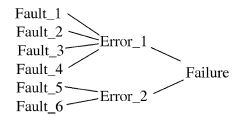
\includegraphics[width=8cm]{content/faulttolerance/images/fault-error-failure-dependency.jpg}
	\caption{Fault->Error->Failure Dependency}
\end{figure}

\subsubsection*{Failures}
 Bei fail-silent Failure wird entweder das korrekte Ergebnis zurückgegeben oder keines. So kann einfach entschieden werden, ob ein Ausfall Einfluss auf andere Systeme hat. Bei korrektem Ergebnis können alle Systeme gleich weiterarbeiten und falls kein Resultat vorliegt, ist der Ausfall eines Systems bekannt und kann entsprechend behandelt werden. Falls beim ersten Auftreten eines fail-silent Failures ein System nicht mehr weiterarbeitet, spricht man von einem crash Failure.

Grob kann man Ausfälle in zwei Gruppen einteilen:

\begin{itemize}
    \item Konsistent: gleiche Bedingungen führen zu gleichem Fehlverhalten, ist aber unabhängig vom Betrachter.
    \item Inkonsistent: Das Fehlverhalten ist abhängig vom Betrachter und von den Bedingungen, gleiche Bedingungen müssen aber nicht zu gleichem Fehlverhalten führen.
\end{itemize}

Fehlertolerantes Design versucht, inkonsistente Fehler in konsistente Fehler umzuwandeln, welche wiederum als fail-silent Failures behandelt werden können.

\begin{figure}[H]
	\centering
	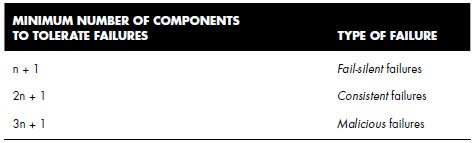
\includegraphics[width=\textwidth]{content/faulttolerance/images/failure-redundancy-num-components.jpg}
	\caption{Minimale Anzahl an Komponenten um Failures auszugleichen}
\end{figure}

\subsection{Coverage}
 Die Absicherung (Coverage) ist die Wahrscheinlichkeit, dass ein System in vorgegebener Zeit einen Fehler automatisch beheben kann.

\subsection{Reliability}

Die Zuverlässigkeit (Reliability) ist die Wahrscheinlichkeit, dass in einem System in vorgegebener Zeit keine Fehler auftreten.

\begin{itemize}
	\item \gls{MTTF} (Mean Time to Failure): Durchschnittliche Zeit vom Starten einer Operation bis zum ersten Ausfall.
	\item \gls{MTTR} (Mean Time to Repair): Durchschnittliche Zeit, die benötigt wird um eine ausgefallene Komponente wieder in einen funktionierenden Zustand zu versetzten.
	\item \gls{MTBF} (Mean Time between Failures): MTTF + MTTR
	\item \gls{FIT} (Failures in Time):  $\frac{Failures}{1e^{9}[h]}$
\end{itemize}

\textbf{Berechnung der Zuverlässigkeit:}
$reliability = e^{-(\frac{1}{\gls{MTTF}})}$

\subsection{Availability}
Die Verfügbarkeit (Availability) ist die Wahrscheinlichkeit in der Zeit, dass ein System erreichbar ist und seine vorgesehenen Aufgaben korrekt erledigen kann.

\begin{figure}[H]
	\centering
	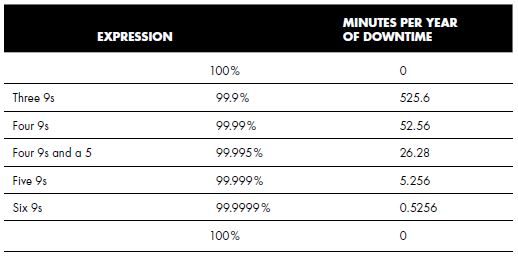
\includegraphics[width=\textwidth]{content/faulttolerance/images/downtime-per-year.jpg}
	\caption{Downtime per year}
\end{figure}

\textbf{Berechnung der Verfügbarkeit:}
$availability = \frac{\gls{MTTF}}{\gls{MTTF} + \gls{MTTR}}$

\subsection{Dependability}

Die Verlässlichkeit (Dependability) ist die Masseinheit für ein System wie stark man sich auf dessen Verlässlichkeit, Verfügbarkeit und Sicherheit verlassen kann. Die Sicherheit wird durch zwei Faktoren beeinflusst. Zu meinem der „Safety“ (Nichtauftreten von Ausfällen, die einen grösseren Schaden anrichten, als der Mehrwert, aller Vorteile eines System, mit sich bringt) und der „Security“ (Verhinderung von unautorisierten Zugriffen/Aktionen).

\subsection{Performance}

Die Leistungsfähigkeit (Performance) ist stark gekoppelt an die Zuverlässigkeit. Anforderungen an die Leistungsfähigkeit, können auch als Anforderungen an die Zuverlässigkeit gesehen werden und umgekehrt. Grundsätzlich kann festgehalten werden, dass Ausfälle, welche auf zu viele Anfragen zurückzuführen werden können, die Leistungsfähigkeit betreffen.

Falls dies geschieht, sind drei mögliche Szenarien möglich:

\begin{itemize}
	\item Crash: Das System bricht unter der Last zusammen
	\item Saturation: Das System läuft weiter, aber mit stark verminderter Leistungsfähigkeit (während der Überlastung) und kehrt schlussendlich wieder zu seiner erwarteten Leistungsfähigkeit zurück.
	\item Capacity decrease: Das System läuft weiter, aber die Leistungsfähigkeit wird dauerhaft vermindert bleiben.
\end{itemize}

\begin{figure}[H]
	\centering
	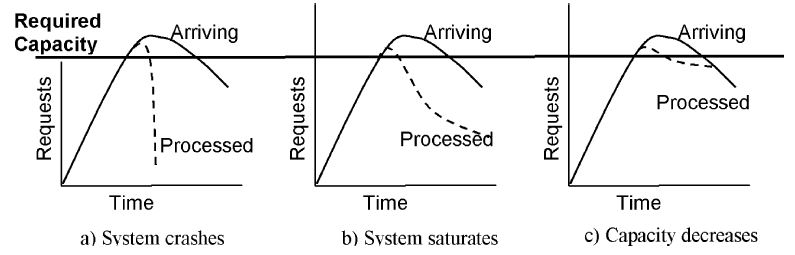
\includegraphics[width=\textwidth]{content/faulttolerance/images/performance.jpg}
	\caption{Performance}
\end{figure}
\section{Fault Tolerant Mindset}

\subsection*{Kontext}


\subsection*{Problem}


\subsection*{Lösung}


\subsection*{Vorteile}
\begin{itemize}
	\item
\end{itemize}

\subsection*{Nachteile}
\begin{itemize}
	\item
\end{itemize}

\subsection*{Reallife Beispiele}
\begin{itemize}
	\item
\end{itemize}

\subsection*{Mögliche Prüfungsfragen}
\begin{itemize}
	\item \emph{Frage?}\\
	Antwort.
\end{itemize}

\section{Introduction to the Patterns}

Die vier Phasen des Lebenszyklus eines Fehlers sind:
\begin{itemize}
	\item error detection
	\item error recovery
	\item error mitigation
	\item fault treatment
\end{itemize}

Diese spielen wie folgt zusammen:

\begin{figure}[H]
	\centering
	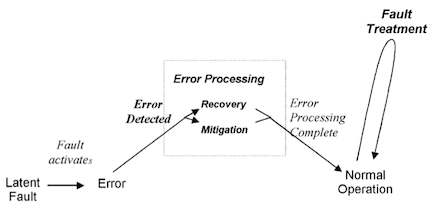
\includegraphics[width=\textwidth]{content/faulttolerance/images/introduction_four_phases_of_fault_tolerance.png}
	\caption{introduction four phases of fault tolerance}
\end{figure}


\subsection{Shared Context for These Patterns}

Die Patterns zielen auf folgende Attribute ab

\subsubsection*{Real-Time}

Zwei unterschiedliche Varianten
\begin{itemize}
	\item soft real-time: Beispiel Webserver antwortet direkt auf Anfrage, ist jedoch nicht schlimm wenn es mal länger dauert
	\item hard real-time: Beispiel Flugzeug, falls ein Kontrollsystem nicht in Echtzeit reagiert kann dies katastrophale Folgen haben
\end{itemize}

\subsubsection*{State or Stateless}

\begin{itemize}
	\item stateless, eine Anfrage wird verarbeitet und ist danach nicht mehr Teil des Systems
	\item stateful, Systeme dessen Verarbeitung längere Zeit in Anspruch nehmen und sich Daten merken müssen
\end{itemize}

\subsubsection*{External Observers}

Oft besitzen Fehlertolerante Systeme Observer bzw. Monitoring Teile welche Informationen über aufgetretene Fehler sammeln. Dies ist eine wichtige Anforderung an das System, da dadurch Fehler analysiert und reduziert werden können.

\subsubsection*{Integrated Fault Tolerance}

Meist ist die Fehlerbehandlung in Programm integriert, dies macht es schwierig eine Fehlerbehandlung in anderen Situationen wieder zu verwenden.

\subsubsection*{Fault Tolerance is Not Free}

Behalte im Hinterkopf das eine Fehlerbehandlung meist nicht gratis ist, z.B. braucht eine redundante Daten Kopie zusätzlichen Speicher.

\subsubsection*{Long Lived Systems}

Lang lebend = höhere Entwicklungskosten = Erwartung das Fehler Tolerant

\subsection{Terminology}

Ein "System" besteht aus "Komponenten" ("Klassen" oder "Module"), diese Komponenten laufen in oder enthalten verschiedene "Tasks", diese wiederum laufen auf eine Einheit von Hard- oder Software. Solange keine Fehler den Verlauf eines Systems stören, nennt man dies "normal processing". Wenn ein System mit unterschiedlichen Komponenten zusammenarbeitet nennt man diese "peers".



\subsection{Fragen}

\begin{enumerate}
	\item Wie heissen die vier Phasen eines Faults?
	\begin{itemize}
		\item error detection
		\item error recovery
		\item error mitigation
		\item fault treatment
	\end{itemize}

	\item Weshalb ist Fault Tolerance nicht gratis?
	\begin{itemize}
		\item Redundanz kostet Speicher
		\item Monitoring kostet Rechenleistung
	\end{itemize}

\end{enumerate}



\section{Units of mitigation}

\subsection{Einleitung}

Dieses, wie auch die folgenden Patterns, zielen auf alle Teile eines Systems ab, und nicht nur auf ein bestimmtes Modul oder eine bestimmte Klasse.

Die Architektur eines Systems hat einen beträchtlichen Einfluss auf die Fehlertoleranz. Deshalb sind die Architectural Patterns auch die ersten, die auf ein neues Projektdesign angewendet werden und sind aus diesem Grund auch die ersten in diesem Buch beschriebenen.

\begin{figure}[H]
	\centering
	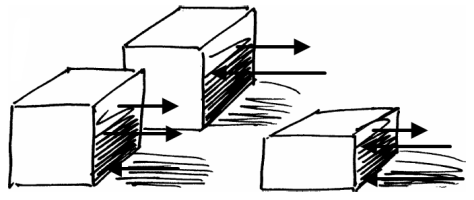
\includegraphics[width=\textwidth]{content/faulttolerance/images/unitsOfMitigation.png}
	\caption{unitsOfMitigation}
\end{figure}

\subsection{Problem}

Wie kann ich verhindern, dass das ganze System ausfällt, sobald irgendwo ein Fehler auftritt? Es sollte möglich sein, dass nur ein Teil ausfällt, den Fehler bestenfalls behebt und sich dann wieder ins System einklinkt.

Dieser eine Teil wird hier 'unit of mitigation' genannt. Wieviele davon das System enthält, und wie gross diese sind, hängt sehr von der jeweiligen Situation ab.

Wie alle Massnahmen zur Fehlertoleranz liefert auch die unit of mitigation ('Einheit zur Schadensmilderung') einen overhead an Code und Komplexität. Sie sollte deshalb nicht zu klein gewählt werden (beispielsweise jeden Ort 'einkapseln', an dem ein Fehler auftreten kann).
Ist sie zu gross, sind wir wieder beim Beispiel, dass das ganze System ausfällt. Es gilt also, einen guten Mittelweg zu finden.

\subsection{Lösung}

\textbf{\textit{Teile das System so ein, dass jeder Teil sowohl mögliche Fehlerquellen wie auch Massnahmen zur Erkennung und Behebung beinhaltet.}} Wähle die Aufteilung so, dass sie für dein System Sinn macht.

Als mögliche, natürliche Trennlinien können in Frage kommen:
\begin{itemize}
	\item Tiers / Layers
	\item Teilapplikationen
	\item Prozessoren, Cores
	\item Threads
	\item Tasks
	\item Terminals / Protokol Handlers
	\item Gruppen von Funktionalitäten
\end{itemize}

Die units of mitigation sollten gegen Aussen genau definierte Interfaces haben. Diese bilden dann eine strikte Barriere für die Fehler und es sollte höchstens bekannt gegeben werden, dass ein solcher aufgetreten ist. Dies bedingt, dass eine Einheit in der Lage sein muss, Fehler zu erkennen und zu beheben.

Das Hinzufügen von Redundanz kann helfen, das System lauffähig zu halten. Ist eine unit damit beschäftigt, einen Fehler zu beheben, kann das redundante Gegenstück einspringen und die Mehrarbeit übernehmen.

Lässt sich ein Modul gut restarten, spricht dies für eine gute Wahl einer unit of mitigation.



\subsubsection*{Correcting Audits}

\subsubsection*{Begriffe}

\subsubsection*{dynamisch vs. statisch}

Daten können dynamisch oder statisch sein. Die Telefonvorwahl eines bestimmten Kantons wird wohl nicht so bald ändern und gehört somit zu den statischen Daten. Der Wechselkurs einer Fremdwährung dagegen ändert sich sehr dynamisch.

\subsubsection*{Problem}

Defekte (faulty) Daten führen zu Fehlern (error). Solche Fehler können und werden immer wieder auftauchen, und müssen auch nicht deterministisch sein. Die Gründe sind vielfältig:
\begin{itemize}
	\item Verfälschung auf Hardware-Ebene: Memory, Strahlung, ...
	\item Andere Systemfunktionen, welche Daten falsch gespeichert haben
\end{itemize}


Dauert die Erkennung des Fehlers zu lange, kann es sein, dass andere Module die Daten nutzen und im schlimmsten Fall das System zum Crashen bringen.

\subsubsection*{Lösung}

\textbf{\textit{Finde und korrigiere defekte Daten so früh wie möglich. Prüfe, ob ähnliche, bzw. zugehörige, Daten auch korrupt sind und protokolliere den Fehlerauftritt.}}

\subsubsection*{Finden und Korrigieren}

Daten können anhand verschiedener Kriterien geprüft werden:
\begin{itemize}
	\item Struktur: Prüfe, ob (double) linked lists korrekt verkettet sind, Pointers auf Listen oder Queues innerhalb der bekannten Grenzen sind, Sizecounters die korrekte Anzahl Elemente angeben, ...
	\item Zusammenhang: Passen gleiche opder ähnliche Daten zueinander? (z.B. könnten Daten an einem Ort in °C gespeichert sein, an einem anderen Ort in °F.)
	\item 'Ergibt das Sinn?': Ein int mit Wert 2013 kann zwar ein gültiges Jahr repräsentieren, aber kaum ein gültiges Jahr. Checksummen können hier helfen, Fehler zu erkennen.
	\item Vergleich: Redundant gespeicherte Daten können direkt miteinenander verglichen und so auf Fehler überprüft werden. Dies macht v.a. für statische Daten Sinn, zum teil aber auch für sehr wichtige dynamische.
\end{itemize}

Daten müssen natürlich so designet werden, dass sie geprüft werden können:
\begin{itemize}
	\item Doppelt verkettete Listen halten die Verkettung redundant
	\item Nutze redundante Speicherorte an verschiedenen Stellen im System
	\item Nutze nicht-triviale Wertevorgaben; Fehler werden so offensichtlicher
\end{itemize}

Verschiedene Patterns helfen, defekte Daten zu korrigieren:
\begin{itemize}
	\item Data Reset
	\item Error Correcting Code
	\item Marked Data
	\item Complete Parameter Check
	\item Rollback
	\item Return To Reference Point
\end{itemize}

Falls die Korrektur erfolgreich war, führe den Schritt noch einmal mit den korrigierten Daten aus.

\subsubsection*{Korrupte Verwandte}

Wurde ein Fehler automatisch gefunden, sollte überprüft werden, ob nicht andere Daten an anderen Orten auch betroffen sind. Möglicherweise entstand der Fehler aus der Berechnung von schon fehlerhaften Daten. Oder der kurrpte Datenbestand wird für die Berechnung weiterer Daten gebraucht. Diese Daten sind potenzielle weitere Fehlerquellen und sollten dann ebenfalls überprüft werden.

\subsubsection*{Protokollieren}

Ein gefundener Fehler sollte immer geloggt werden. Wiederholte Auftritte von Fehlern können helfen, die defekten Daten zu finden.

\subsection{Escalation}

\begin{figure}[H]
	\centering
	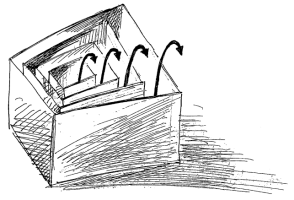
\includegraphics[width=\textwidth]{content/faulttolerance/images/escalation.png}
	\caption{escalation}
\end{figure}

\subsubsection*{Problem}

Trotz allen Versuchen kann es sein, dass sich das System im Fehlerfall nicht wiederherstellen kann. Sowohl Correcting Audits, als auch Restarts, Data Resets und Rollback- oder Rollforwardversuche verlaufen manchmal erfolglos. In einigen Fällen kann es genügen, diese Versuche wiederholt anzuwenden, bis das gewünschte Ergebnis erzielt ist. Doch wie bei einer beschädigten LP, die immer wieder dieselbe Stelle wiederholt, ist manchmal drastischeres Eingreifen gefragt. Da das System das Prinzip von Minimize Human Intervention verfolgt, soll es dafür aber selbst verantwortlich sein.

\subsubsection*{Lösung}

\textbf{\textbf{Wenn Fehlerkorrektur und -abschwächung fehlschlagen, führe die nächst drastischere Massnahme aus.}}

Es kann nützlich sein, einen Zähler zu haben, damit das System weiss, wie oft ein Wiederherstellungsversuch in welcher Zeit schon fehlgeschlagen ist. Wird ein gewisser Wert überschritten, kann die Eskalation in die nächste Phase ausgelöst werden.

\subsubsection*{Menschliches Eingreifen}

Ab einer bestimmten Phase wird menschliches Eingreifen unumgänglich. Dem Operator muss dann aber eine Liste mit möglichen Schritten vorliegen. Diese sollte so geordnet sein, dass zuerst Massnahmen ausgeführt werden, welche eine hohe Recoverywahrscheinlichkeit haben, aber gleichzeitig schnell sind und einen minimalen Einfluss auf andere Systemoperationen haben. Später folgen dann die schwereren Geschütze.


\subsection{Redundancy}


\subsubsection*{Definition}


Redundanz bedeutet, dass man über zusätzliche bzw. andere Wege verfügt, um die gleiche Arbeit zu verrichten.

\subsubsection*{Einleitung}

Es gibt zwei Arten wie Errors mit Hilfe von Redundanz behandelt werden können; Mit einigen Verfahren gelingt es, Errors zu behandeln ohne den Systemzustand zu ändern (z.B. Block code). Normalerweise ist dies jedoch nicht möglich und erst nach der Behandlung des Errors kann das System wieder in einen fehlerfreien Zustand überführt werden.

Für beide Arten der Fehlerbehandlung kann Redundanz helfen, einen solchen Error zu behandeln bzw. dessen Auswirkungen so gut wie möglich zu überbrücken. (MTTR)

\subsubsection*{Typen von Redundanz}

\subsubsection*{Spatial}

Von räumlicher Redudanz spricht man, wenn von einem System mehrere Kopien existiren. Die Zeit welche zwischen dem Erkennen des Fehlers bis zur Rückführung in einen fehlerfreien Zustand verstreicht, wird als „Recovery Time“  bezeichnet. Räumlich redundante Systeme können diese Zeit mit einer fehlerfreien Kopie des Systems überbrücken.

Beispiel: Nameserver (DNS), RAID1, N-Version Programming

\subsubsection*{Temporal}

Zeitliche Redundanz, wobei die Redundanz über eine Zeitdauer vorhanden ist, um korrekte Resultate zu erhalten. (Nachteil: Unavailability kann erhöht werden)

Beispiel: I-frame ( http://en.wikipedia.org/wiki/I-frame )

\subsubsection*{Informational}

Informatorische Redundanz, wobei Information zur Erkennung und Behebung von Fehlern wiederholt wird.

Beispiel: Block Code

\subsubsection*{Methoden für Temporal Redundancy}


\subsubsection*{Active-Active}

Vollständig Redundante Systeme agieren parallel und teilen sich die Arbeit (Load Balancing). Trotzdem ist jedes System fähig die gesamte Arbeit alleine zu verrichten.

\subsubsection*{Active-Passive}

Eine Abwandlung von Active-Active wobei das zweite/"redundante" System erst beim Auftreten eines Errors die Arbeit übernimmt.

\subsubsection*{N+M Redundancy}

Active-Active bzw. Active-Passive setzen eine teure 1:1-Assoziation zwischen den Systemen voraus. N+M Redundancy reduziert die Kosten indem für N aktive Systeme M redundante Systeme bestehen, wobei M < N

\subsubsection*{Tradeoff}


Redundanz bedeutet auch immer einen Mehraufwand und somit höhere Kosten. Ausserdem handelt es sich bei Computern um deterministische Maschinen welche bei gleichen Rahmenbedingungen, Konfiguration und Input auch gleichermassen auf Fehlsituationen reagieren.

\subsubsection*{Prüfungsfragen}

\begin{itemize}
	\item Definieren Sie den Begriff Redundanz.
	\item Nennen Sie je ein Beispiel für Spatial, Temporal und Informational Redundancy.
	\item Unterscheiden Sie die Begriffe Active-Active, Active-Passive und N+M Redundancy.
\end{itemize}

\begin{itemize}
	\item Unterscheiden Sie die Begriffe Active-Active, Active-Passive und N+M Redundancy.
\end{itemize}


\subsection{Recovery Blocks}


\subsubsection*{Einleitung}

Im Kapitel \url{http://wiki.ifs.hsr.ch/APF/U11_3_Redundancy} wurde bereits darauf hingewiesen, dass eine exakte Kopie auch die gleichen Fehler produzieren wird. Daher müssen alternative Lösungen für eine Problemstellung unterschiedlich implementiert werden. Dies kann wie folgt bewerkstelligt werden
\begin{itemize}
	\item Redundante Implementierungen parallel ausgeführt. Mittels Voting wir anschliessend das beste Resultat gewählt. (Nachteil: Overhead)
	\item Alternative werden nur ausgeführt, wenn das erste Resultat nicht befriedigend war, die ist die Recovery Block Strategie.
\end{itemize}

\subsubsection*{Beispiel}

\begin{verbatim}
  Try
    Heap sort
    if not okay then throw
  Catch
    Try
      Insertion sort
      if not okay then throw
    Catch
      Bubble sort
\end{verbatim}

\subsubsection*{Tradeoff}

\begin{itemize}
	\item Akzeptanz-Tests: Es ist nicht immer einfach zu entscheiden ob ein Resultat akzeptiert werden kann.
	\item Alternativen: Für gewisse Algorithmen gibt es keine oder nur unbefriedigende Alternativen.
	\item State: Der System State muss vor dem ersten Block gespeichert werden, damit für den nächsten Block die gleichen Bedingungen herrschen.
	\item Komplexität: Recovery Blocks an sich führen zu mehr Code und somit zu mehr Komplexität. Auch die vorherigen Punkte tragen zu einer höheren Komplexität bei.
\end{itemize}

\subsubsection*{Prüfungsfragen}

\begin{itemize}
	\item Um welchen Typ von Redundanz handelt es sich bei Recovery Blocks?
	\item Stellen Sie die Funktionsweise von Recovery Blocks anhand von Pseudocode und einem Fluss-Diagramm dar.
	\item Nennen Sie drei Nachteile von Recovery Blocks.
\end{itemize}

\begin{itemize}
	\item Nennen Sie drei Nachteile von Recovery Blocks.
\end{itemize}



\subsection{Minimize Human Intervention}

\subsubsection*{Ausgangslage}

Für viele Fehler in Systemen sind deren Benutzer verantwortlich, da sie mit falscher Anwendung diese provozieren.
\subsubsection*{Lösungsansatz}

Es gibt drei Kategorien von Fehler in Systemen:
\begin{enumerate}
	\item Hardware
	\item Software
	\item Prozedurale
\end{enumerate}


\subsubsection*{Vergessene Aktionen}

Grundsätzlich verhalten sich Personen schlechter als Computer, wenn sie immer dieselben Schritte (Prozeduren) durchlaufen müssen. Ein Computer haltet sich strikt an die vorgegebene Reihenfolge (ausser Ausnahmen sind explizit zugelassen), eine Person hingegen kann einzelne Schritte überspringen, sei das nun weil sie diesen vergessen oder absichtlich nicht erledigt hat. Läuft ein System fehlerfrei, dann wird diesem System weniger Aufmerksamkeit geschenkt, und dabei können wichtige Aktionen vergessen gehen, falls diese dennoch erwartet werden.
Tritt ein Fehler auf, kann ein Computer viel schneller reagieren als eine Person, die das System bedient.

\subsubsection*{Unerlaubten Aktionen}

Es kann aber auch vorkommen, dass eine Person denkt, dass ein System nicht mehr richtig funktioniert, obwohl dies nicht der Fall ist. Dieser Umstand ist darauf zurückzuführen, dass einer Person nicht genügend Feedback gegeben wird, dass ein System noch am Arbeiten ist. Die einfachste Form hierfür ist eine Progressbar oder die animierten Mauszeiger, welche aus den Betriebssystemen bekannt ist.
Im Allgemeinen gilt: „A quite system is a dead system“
Tritt diese Situation ein, kann es sein, das seine Person Aktionen auslöst, die nicht erwartet werden und die Situation meist verschlechtern. So kann sie einen einwandfrei laufenden Prozess abschalten oder weitere Prozesse starten, die das System noch mehr auslasten.


\subsubsection*{Schlussfolgerung}

Ein System soll so designet werden, dass es selbst Fehler behandeln und automatisch wieder einen normalen Zustand erreicht. Dies führt zu einer schnelleren Fehlerbehandlung, kürzerer Ausfallzeit und es wird vermieden, dass Prozedurale-Fehler während der Behandlung eines Fehlers auftreten können.

\begin{figure}[H]
	\centering
	
\includegraphics{content/faulttolerance/images/MinimizeHumanIntervention.JPG}
	\caption{MinimizeHumanIntervention}
\end{figure}


Erreicht kann dies wie folgt werden:
\begin{enumerate}
	\item Fehler müssen einem Fault Observer (10) gemeldet werden.
	\item Es dürfen keine internen Meldungen nach aussen gesandt werden.
	\item Die Unit of Mitigation (1) soll Fehler selbst erkennen, behandeln und beheben können, ohne dafür auf Interaktion mit einer Person angewiesen zu sein.
\end{enumerate}

Fehlerbehandlung:
\begin{itemize}
	\item Recovery Blocks (4)
	\item Error Handler (30)
\end{itemize}

Vermeidung von Prozeduralen-Fehlern:
\begin{itemize}
	\item Maximize Human Participation (6)
	\item Maintainance Interfaces (7)
	\item Reintegration (59)
	\item Revise Procedure (63)
\end{itemize}


\subsection{Someone In Charge}

\subsubsection*{Ausgangslage}
Ein System besteht aus mehreren Units of Mitigation (1), kann Redundancy (3) verwenden und verfolgt das Prinzip von Minimize Human Interaction (5).
Dennoch können überall Fehler auftreten, selbst in der Fehlerbehandlung. Tritt dieser Fall ein, kann es sein, dass das System, zusätzlich zum Ausfall der Funktionalität auch noch die Fehlerbehandlung nicht weiterführen kann.

\subsubsection*{Lösungsansatz}

Bei der Fehlertoleranz gibt es zwei Arten der Fehlererkennung:
\begin{enumerate}
	\item Fehler erkennen, der passiert ist (komplexer)
	\item Die Komponente im System finde, welche nicht mehr korrekt funktioniert (einfacher)
\end{enumerate}
Hat ein System eine Komponente, die weiss was bei der Erkennung eines Fehlers gemacht werden muss, führt das zu einem robusteren System. Mindestens sollte diese den Fehler einem Fault Observer (10) oder System Monitor (15) melden können, nebst einer möglichen Fehlerbehandlung. Ein Fault Observer (10) ist zuständig für das Sammeln und Weiterleiten von Informationen von Fehlern, ein System Monitor (15) hingegen erkennt Fehler.
Wichtig ist einfach, dass im Falle eines Fehlers bekannt ist, wer sich darum kümmern muss.
Das Problem dabei ist aber, dass dadurch ein Single Point of Failure entsteht, da diese Komponente auch ausfallen kann. Es ist deshalb nicht definiert, dass es nur eine Komponente geben darf, die reagieren kann. Es ist lediglich definiert, dass zu jedem Zeitpunkt klar sein muss, wer reagieren muss.
Wichtig ist auch zu beachten, dass die verantwortlichen Komponenten sich nicht um zu viel kümmern müssen. Es ist einfacher, wenn sich viele verschieden Komponenten um verschieden Fehlerbehandlungen kümmern, da diese so einfacher wartbar sind und bei einem Ausfall einer Komponenten nicht die gesamte Fehlerbehandlung betroffen ist.

\begin{figure}[H]
	\centering
	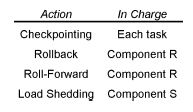
\includegraphics{content/faulttolerance/images/ResponsibilitiesList.JPG}
	\caption{ResponsibilitiesList}
\end{figure}


\subsubsection*{Schlussfolgerung}

Alle Aktivitäten, die fehlertolerant sein müssen, benötigen eine einzige Komponente, die in einem Fehlerfall reagiert.
Es muss auch möglich sein, dass Fehler bei der Fehlerbehandlung erkannt werden können und falls nötig Escalation (9) eingesetzt wird.

\subsubsection*{Verwandte Patterns}

Fehler-„Verwaltung“:
\begin{itemize}
	\item Fault Observer (10)
	\item System Monitor (15)
\end{itemize}

\begin{itemize}
	\item Heartbeats (16)
	\item Acknowledgements (17)
\end{itemize}

\begin{itemize}
	\item Escalation (9)
\end{itemize}


\subsection{Maximize Human Participation}

\subsubsection*{Ausgangslage}

Soll ein System Anwender total ignorieren, um die prozeduralen Fehler zu minimieren?

\subsubsection*{Lösungsansatz}

Das System soll dem Benutzer die Möglichkeit bieten das Systems bei der Fehlerbehandlung zu unterstützen. Beispielsweise versucht das System immer wieder mit einem ROLLBACK zu einem CHECKPOINT (37) zu springen, obwohl der Speicher, an dem der CHECKPOINT gespeichert wurde, beschädigt ist. Der Benutzer könnte nun das System dazu zwingen einen RESTART (31) durchzuführen, anstatt eines ROLLBACK (32).

Wichtig ist dem Benutzer die wichtigsten Systeminformation zu präsentieren. Dabei soll darauf geachtet werden, dass weniger wichtige Informationen nach den kritischen Informationen folgen. Nachrichten, welche Fehler melden, werden im Fault Tolerance Bereich als 'Action Messages' bezeichnet.

Das System sollte weiter einen 'Safe Mode' bieten, in welchem es keine weiteren automatischen Fehlerbehandlungen vornimmt. Dies ist vor allem in Kritischen System sehr wichtig.

\subsubsection*{Schlussfolgerung}

Ein System soll so designet werden, dass es für erfahrene Benutzer einfach ist in einem positiven Weg auf das laufende System einzuwirken. Hierzu kann ein gutes MAINTANCE INTERFACE (7) und ein gescheiter FAULT OBSERVER (10) hilfreich sein.

Ebenfalls wichtig für die Stabilität des Systems ist es, nach einem Error eine ROOT CAUSE ANALYSIS (62) durchzuführen, um mögliche Ursachen zu identifizieren und falls nötig ein SOFRWARE UPDATE (11) einzuspielen.


\subsection{Maintenance Interface}

\subsubsection*{Ausgangslage}

Sollen Wartungs- und Anwendungsanfragen in den Ein- und Ausgangskanälen des Systems vermischt werden?

\subsubsection*{Lösungsansatz}

Es sollte ein eigenes Interface für Wartungsanfragen zur Verfügung gestellt werden. Wobei diese Anfragen priorisiert werden und in der Anwendung auch bei Überlast abgearbeitet werden, wodurch das Wartungspersonal immer in der Handlungsmacht ist. Des Weiteren bringt dies eine höhere Abschottung mit sich, da es aus der 'normalen' Applikation nicht möglich ist in den Wartungsmodus zu gelangen. Ebenfalls kann dieses Interface mit nötigen Security Features geschützt werden.

\subsubsection*{Schlussfolgerung}

Stellen sie ein eigenes Interface für die exklusive oder fast exklusive Möglichkeit für Wartungsarbeiten zur Verfügung.



\subsection{Fault Observer}

\subsubsection*{Ausgangslage}

Das System ist so designt das es Fehler entdeckt und automatisch behandelt und löst. Wie erfahren nun Personal oder andere Systemkomponenten von einem möglichen Problem?

\subsubsection*{Lösungsansatz}

Der herkömmliche Ansatz ist das PUBLISHER-SUBSCRIBER Pattern, welches einen effektiven Weg zur Verteilung von aufgetretenen Fehler darstellt. Hierbei registrieren (subscriben) sich die Observer für Informationen/Komponenten. Sobald neue Informationen oder Fehler eintreffen werden diese an die registrierten Observer weiterverteilt.

\begin{figure}[H]
	\centering
	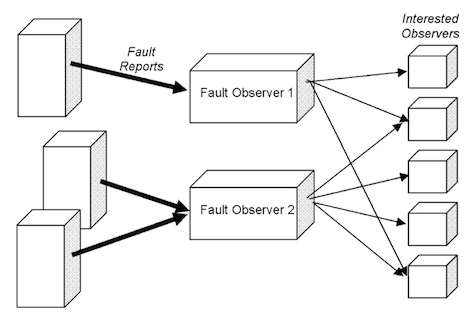
\includegraphics[width=\textwidth]{content/faulttolerance/images/U11_3_FaultObserver_2013.png}
	\caption{U11 3 FaultObserver 2013}
\end{figure}


Wichtig ist darauf zu achten das die Publisher einmalig oder als redundante Komponenten vorhanden sind und nicht mehrere Publisher die den selbe Information an einen Observer übermitteln. (führt zu Konfusion beim Observer und zu duplicated Code im System) Des Weiteren wäre es wünschenswert, dass bei einem Error der dazugehörige Fault mit geloggt wird um spätere Analysen zu vereinfachen.

\subsubsection*{Schlussfolgerung}

Raportiere alle Errors an einen Fault Observer, welcher alle intressierten Parteien darüber informiert.


\subsection{Software Update}

\subsubsection*{Ausgangslage}

Trotz guter Qualitätssicherungsmethoden zur Vermeidung von Fehlverhalten kann es zu Fehlern kommen. Wodurch Software Updates nötig werden, diese dürfen jedoch das System nicht zu Anhalten zwingen und die damit verbundene Downtime minimieren.

\subsubsection*{Lösungsansatz}

Vor der ersten Applikationsauslieferung muss geklärt sein wie sie erweitert bzw. erneuert werden kann, ohne das System zu stoppen.

Falls die neue Version einer Applikation zur gleichen Zeit wie die alte ausgeführt werden kann, ist es möglich einen Failover Routine laufen zu lassen die zwischen der alten und der neuen Version interagiert. Dies ermöglicht eine minimale Downtime. Zudem können automatisierte Akzeptanztests gestartet werden, welche prüfen ob die neue Version korrekt arbeitet. Falls dies nicht der Fall ist, kann mittels Recovery Blocks wieder zur alten Version zurück gewechselt werden.

In einem komplexen System können nicht alle Komponenten des Systems gleichzeitig ausgetauscht werden. Es kann also erforderlich sein, dass das neue Komponenten rückwärtskompatibel sein müssen. Dies kann unter anderem erreicht werden, indem ein Versionsindikator eingeführt wird und die neuen Funktionen Regeln enthalten, welche festlegen wie sie mit fehlenden oder geänderten Attributen umgehen soll.

\subsubsection*{Schlussfolgerung}

Designen sie die Applikation so, das Änderungensmöglichkeiten bereits in ihrerem ersten Release miteingeflossen sind. Halten sie sich immer vor Augen wie sie die Software im ausgelieferten Zustand erweitern und verbessern können, da ein einbauen einer Update Routine nachdem Ausliefern keine einfache Sache ist.


\section{Detection Patterns}


Die erste Phase von Fault Tolerance ist Entdeckung. Faults und daraus resultierende Errors müssen erst erkannt werden, bevor Recovery- oder Schadensminderungsaktionen etc. ausgeführt werden können.

Zwei Paare von Konzepten sind dabei wichtig: 'Errors' vs. 'Failures' und 'a priori Wissen' vs. 'Vergleich von redundanten Elementen'.
\begin{figure}[H]
	\centering
	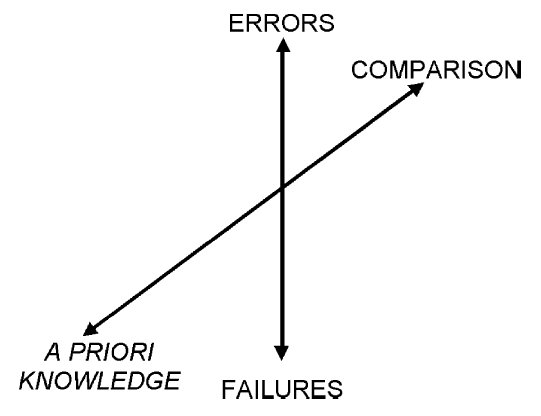
\includegraphics[width=\textwidth]{content/faulttolerance/images/detection_concepts.png}
	\caption{detection concepts}
\end{figure}


\subsection*{'a priori Wissen' vs. 'Vergleich von redundanten Elementen'}


Wir können Wissen über das System und darin geltende Constraints nutzen um zur Laufzeit Zustände, Resultate, Seiteneffekte etc. überprüfen zu können.

Die meisten Patterns nutzen eher den zweiten Ansatz, wie z.B. REDUNDANCY(4).

Ein weiterer Aspekt wäre, dass das Programm selbst in der Lage ist, zu erkennen, dass (und welche) Fehler immer wieder auftauchen und so automatisch Errors und Failures erkennt.

\subsection*{'Errors' vs. 'Failures'}


Das System muss in der Lage sein, sowohl Errors als auch Failures zu erkennen. Wir sind natürlich v.a. an den Errors interessiert, da diese die "Wurzel der Probleme" sind. Bestenfalls finden wir sie, wenn sie noch gar nie im System Schaden anrichten konnten.

\begin{figure}[H]
	\centering
	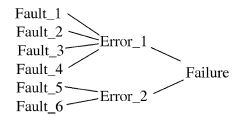
\includegraphics{content/faulttolerance/images/FaultErrorFailureDependency.JPG}
	\caption{Fault Error Failure Dependency}
\end{figure}


\subsection*{Übersicht über die Patterns im folgenden Kapitel}


\begin{figure}
	\centering
	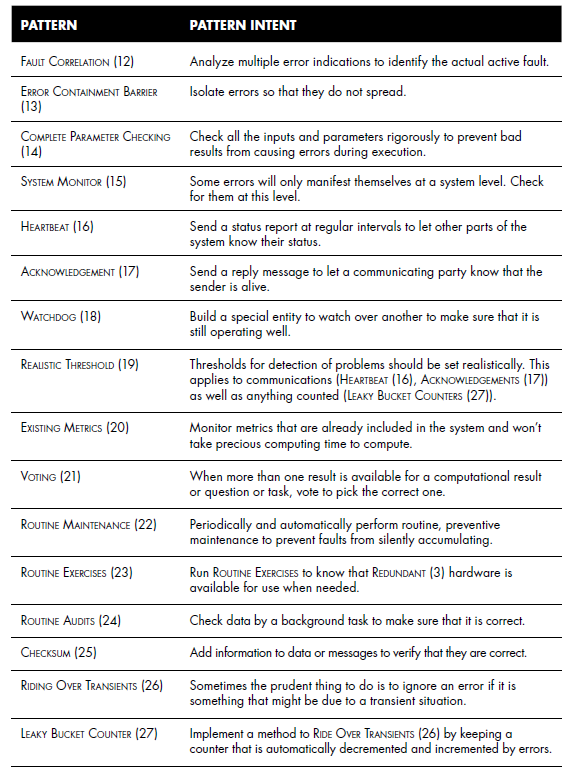
\includegraphics{content/faulttolerance/images/pattern_thumbnails.png}
	\caption{pattern thumbnails}
\end{figure}


\begin{figure}
	\centering
	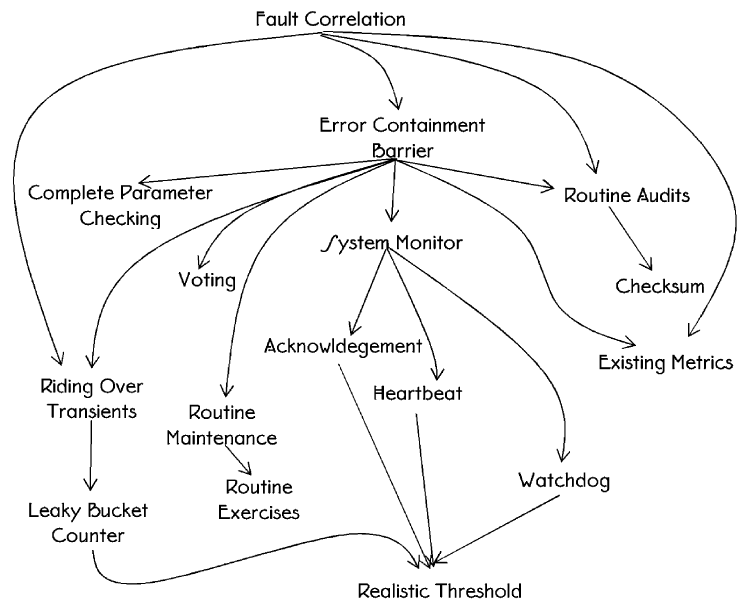
\includegraphics[width=\textwidth]{content/faulttolerance/images/pattern_map.png}
	\caption{pattern map}
\end{figure}




\subsection{Fault correlation}


\subsubsection*{Problem}

Ein Fehler ist aufgetreten und wurde detektiert. Es gibt aber viele verschiedene mögliche Ursachen.
Die Frage lautet nun: Welcher Fault führte zum Fehler?

\subsubsection*{Lösung}


Ein Error oder Failure kann von diversen Faults ausgelöst werden. Beim Auftritt eines Fehlers sollten diverse Fragen gestellt werden, wie z.B.:
\begin{itemize}
	\item Was hat der Fehler im System schon angestellt?
	\item Wurde die Ausführung gestoppt? Wenn ja, welche Funktionen sind nicht mehr verfügbar?
	\item Wurden Logs erstellt?
	\item Welche Daten waren nicht korrekt?
	\item ...
\end{itemize}

Die ursprüngliche Fehlerquelle zu finden ist extrem wichtig!
\begin{itemize}
	\item Ein Error kann weitere Errors verursachen.
	\item Ähnliche Errors oder Failures könnten evtl. die gleiche Behandlungsprozedur besitzen. So kann z.B. in einem Redundanten System auf eine andere Komonente ausgewichen werden und die Fehlerbehebung hat noch etwas Zeit. Andererseits kann es sein, dass der Fehler so schnell wie möglich behoben werden muss, damit das System nicht davon 'verseucht' wird.
\end{itemize}

Um letzteres zu ermöglichen, sollten gewisse Bug-Kategorien erstellt werden, damit klar ist, wie mit einem entdeckten Fault umgegangen werden muss.

\subsection{Error containment barrier}


\subsubsection*{Problem}


Was soll das System als erstes tun, wenn ein Error detektiert wird? Ohne Behandlung wird er für immer im System bleiben oder aber früher oder später in einem Failure enden. Was genau geschehen wird kann allerdings selten genau vorausgesagt werden.

Was aber soll getan werden? Eine Möglichkeit ist, 'HILFE' zu schreien und zu beenden, was aber MINIMIZE HUMAN INTERVENTION widerspricht (kann aber nötig sein, wenn sicherheitskritische Fehler geschehen). Den Fehler weitestgehend zu ignorieren ist auch nicht immer die beste Lösung. Es ist auch nicht immer möglich, schadensbegrenzende Schritte (CORRECTING AUDITS etc.) einzuleiten.

Bis sie jemand stoppt, breiten sich Errors durch das System von Komponente zu Komponente aus.

\subsubsection*{Lösung}

Der Error muss in einer UNIT OF MITIGATION isoliert und der Fluss in andere Teile des Systems mit einer Barriere gestoppt werden (Stichwort QUARANTINE).

Der Error darf nicht unbehandelt bleiben. Löse parallel dazu geeignete Benachrichtigungen, Logging, Mitigation und Recovery Funktionen aus.

\subsection{Riding over transients}


\subsubsection*{Problem}


Einige Probleme treten nur sehr selten bis einmalig auf. Eine Bodenwelle bringt den Stossdämpfer kurzzeitig in Unruhe, sonst ist aber meist nicht viel los. Genau so können in Software Fehler selten auftreten und nur kurzzeitig eine Auswirkung haben (Rauschen auf einem Bus, Alphateilchen, ...). Wie kann man jetzt verhindern, dass das System für solche transiente Fälle unnötig viele Ressourcen verbraucht?

\subsubsection*{Lösung}


Führe FAULT CORRELATION durch, wenn ein Fehler auftritt. Kann er keiner Kategorie zugeordnet werden, so beginne sofort mit der Fehlerbehandlung. Sieht er wie ein transienter Fehler aus, so rapportiere den Auftritt und unternimm nur etwas, wenn die Auftrittsfrequenz unerwartet hoch ist.

"Unerwartet hoch" kann natürlich je nach Anwendungsfall unterschiedlich verstanden werden. Wenn andere Daten in Mitleidenschaft gezogen werden muss schneller gehandelt werden, als z.B. bei Web Requests.

Geduld ist eine Kunst! Nicht immer sind die ersten Hinweise die echte Unterschrift eines Errors, weshalb zu frühes Handeln zu falschen Aktionen führen kann.

Beispiele von riding over transients:
\begin{itemize}
	\item Ignorieren des Rückgabewerts bei Festplatten Schreibvorgängen
	\item Laden einer Webpage schlägt fehl. "Versuchen Sie es später noch einmal"
\end{itemize}


\subsection{Leaky bucket counter}


\subsubsection*{Problem}


Wie kann ein System wissen, ob ein Error transient oder sporadisch auftritt? Auch nicht-dauerhafte Fehler können zu Failures führen, sind aber ihrer transienten Natur entsprechend schwierig bis gar nicht zu isolieren und korrigieren.

Oft greift man bis zu einer bestimmten Anzahl selten auftretender Fehler gar nicht ein. Treten sie aber gehäuft ein, so soll das System eine gewisse Fehlerbearbeitung auslösen.

\subsubsection*{Lösung}


Jede zu überwachende UNIT OF MITIGATION bekommt einen LEAKY BUCKET COUNTER. Tritt ein, als transient betrachteter, Fehler auf, wird der Counter inkrementiert. Periodisch wird er aber auch dekrementiert, allerdings nie unter den Anfangswert. Erreicht der Counter nun einen vorgegebenen Threshold, wird der Fehler nicht mehr als transient, sondern als permanent betrachtet.

Die Rate, mit welcher der Bucket geleert wird, muss sorgfältig gewählt werden. Geschieht es zu oft, so werden nicht-transiente Errors gar nie identifiziert.

\begin{figure}[H]
	\centering
	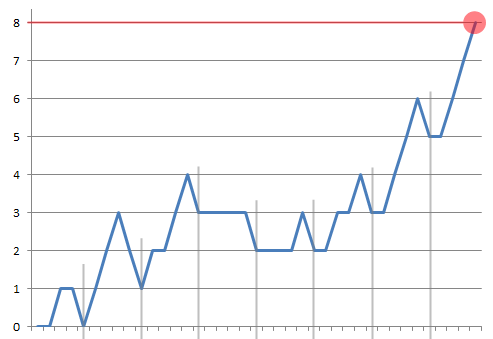
\includegraphics[width=\textwidth]{content/faulttolerance/images/leaky_bucket_counter.png}
	\caption{leaky bucket counter}
\end{figure}




\subsection{Error Recovery Patterns}


\subsubsection*{Einleitung}


Im vorherigen Kapitel haben wir Error Detection kennengelernt; Patterns die Errors erkennen, diese aber nicht (selber) behandeln. Beim Error Recovery geht es darum, nachdem ein Fehler detektiert wurde,, das System wieder in einen fehlerfreien Zustand zurück zu führen. Bei den nachfolgenden Patterns handelt es sich um Vorgehensweisen, ein System wieder in einen Zustand zu bringen, der nicht durch den Error beeinträchtigt wird (auch wenn der Fehler noch im System präsent ist). Man kann aber auch einen fehlerfreien Zustand erreichen, wenn man den Fehler maskiert und soweit abschwächt, dass er nicht mehr als Fehler gezählt werden muss. Patterns für diesen Ansatz werden später noch behandelt.

Bei den nachfolgenden Patterns geht es in erster Linie darum, eine grösstmögliche Verfügbarkeit zu erreichen. Das heisst, dass man beim Auftreten eines Fehlers diesen nicht explizit korrigiert sondern einfach in einen fehlerfreien Zustand springt. Als Folge davon verwenden viele Patterns Checkpoints um Zustände zu speichern um gegebenenfalls zu diesen zurückzukehren. Um eine hohe Availability zu gewährleisten bieten sich der Einsatz von Error Recovery Patterns vor allem in redundanten Systemen an.

\subsubsection*{Übersicht}


Die untenstehenden Error Handler führen das System nach erfolgreicher Fehlerdetektion in einen fehlerfreien Zustand zurück.

\subsubsection*{Error Recovery Patterns - Dependency}

\begin{figure}[H]
	\centering
	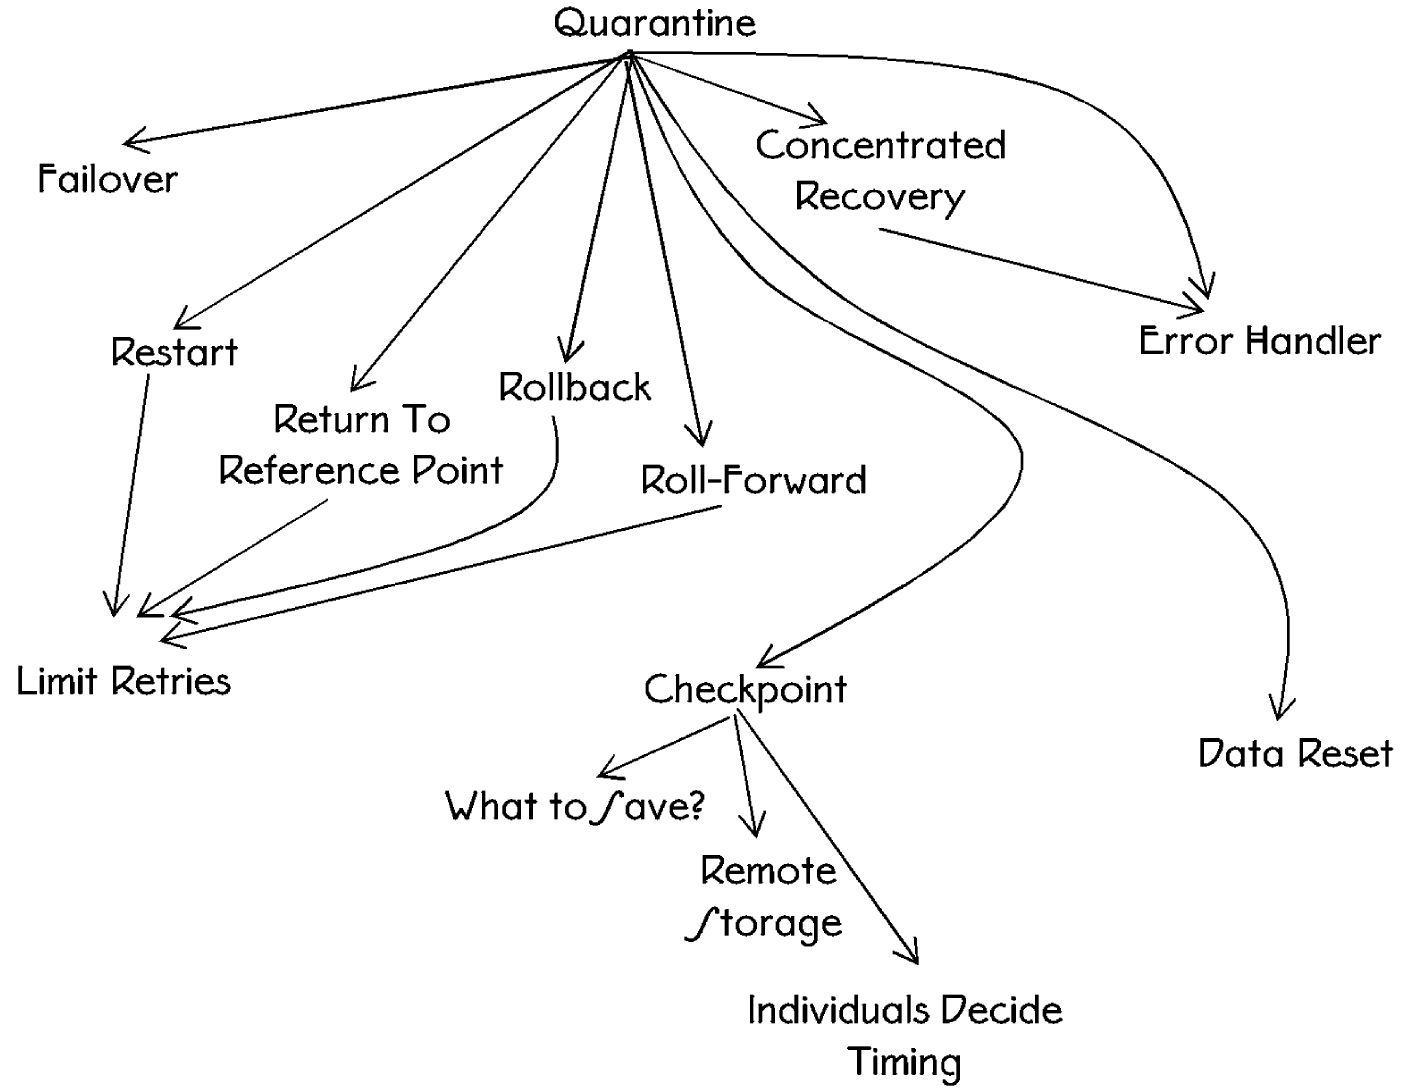
\includegraphics[width=\textwidth]{content/faulttolerance/images/RecoveryPatterns_Dependency.JPG}
	\caption{RecoveryPatterns Dependency}
\end{figure}


\subsubsection*{Error Recovery Patterns - Buch}

\begin{figure}[H]
	\centering
	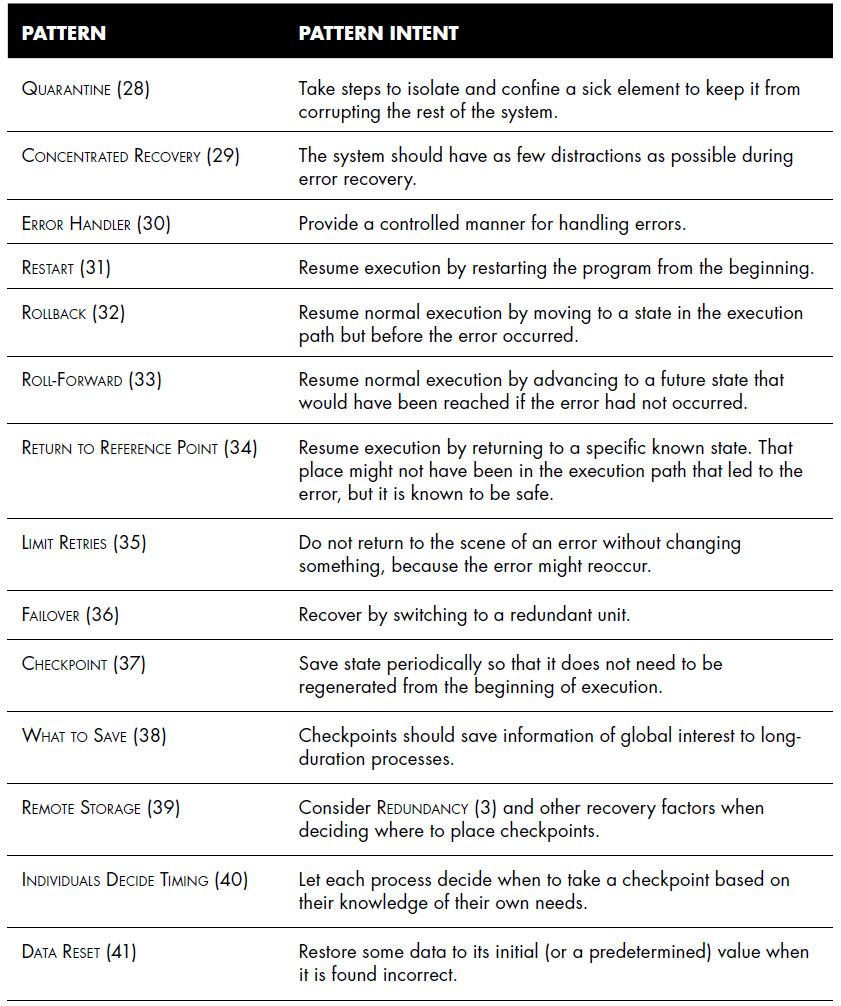
\includegraphics[width=\textwidth]{content/faulttolerance/images/RecoveryPatterns.JPG}
	\caption{RecoveryPatterns}
\end{figure}


\subsubsection*{Prüfungsfragen}

\begin{itemize}
	\item Erklären Sie den unterschied zwischen Error Detection und Error Recovery
	\item Was ist das Ziel, wenn ein Error Handler ``zum Einsatz'' kommt?
\end{itemize}


\subsection{Restart}


\subsubsection*{Problem}


Ein schwerwiegender Fehler wurde detektiert und kein Mechanismus kann bzw. konnte den Fehler beheben; D.h. alle Schritte der Escalation haben versagt. Wie kann das System wieder in einen fehlerfreien Zustand zurück geführt werden?

\subsubsection*{Lösung}


Als letzte Möglichkeit für einen Software-Fehler, der mittels Escalation nicht behoben werden konnte, kann das System neu gestartet werden. Dieser radikale Ansatz wird Restart genannt. Ein Restart hilft aber nur, wenn es sich um ein Software-problem handelt. z.B. Bei einem Hardwarefehler würde der Fehler auch dem Restart im System erhalten bleiben.

Nachfolgeden Patterns sehen Sprünge zu fehlerfreien Zuständen vor wie Roolback, Roll-Forward  und Return to Reference Point. Restart hingegen setzt alles auf den initialen Zustand zurück. Da dies aber der grösste Sprung und meist auch der zeitaufwändigste ist, sollte dieser nur wenn nötig ausgeführt werden. Es gibt auch die Möglichkeit, den Restart in verschiedene Stufen zu unterteilen. Eine mögliche Unterteilung wäre:

\begin{itemize}
	\item warm: Es werden nur gewisse Teile des Systems initialisiert (bei den Teilsystemen, welche nicht neu gestartet werden, wird davon ausgegangen, dass sie noch einwandfrei funktionieren).
	\item cold: Das komplette System wird neu gestartet (nicht aber die Umgebung).
	\item reload: Das System wird neu in den Speicher gelesen und dann gestartet.
	\item reboot: Die Umgebung, auf der das System läuft, wird komplett neu gestartet.
\end{itemize}

Der „warm“ Restart wird meist bei transienten Fehlern verwendet, da diese mit grosser Wahrscheinlichkeit nicht nochmals auftreten werden und nicht das gesamte System betroffen ist.

\subsubsection*{Beispiel}


\begin{itemize}
	\item Bluescreen seit Windows XP
\end{itemize}

\subsubsection*{Tradeoff}


\begin{itemize}
	\item Cold reloads/reboots können zu inkonstistenten Daten führen.
	\item Sehr zeitaufwendig (Downtime/Availability)
\end{itemize}

\subsubsection*{Prüfungsfragen}

\begin{itemize}
	\item Nennen Sie drei verschiedene Stufen des Restarts?
\end{itemize}


\subsection{Roll Back}


\subsubsection*{Problem}


Ein Fehler ist aufgetreten und behandelt worden. Da das System keinen Input ignorieren soll, muss es nach erlangen eines fehlerfreien Zustandes "angestaute" Requests/Messages verarbeiten. Wie soll das bewerkstelligt werden?

\subsubsection*{Lösung}


Das System kann an eine Position zurückspringen, an der bekannt ist, dass der Fehler noch nicht aufgetreten ist. Dies ist meist der Anfang der aktuellen Verarbeitung oder ein Punkt, wo alle Komponenten synchronisiert werden/synchron sind.

Um nicht zu grosse Sprünge in Kauf zu nehmen, können mittels Checkpoints die Distanzen und somit die erneut auszuführenden Aktionen minimiert werden. Dies erfordert aber den grösseren Aufwand bei der Speicherung von Zustandsinformationen.

Wird ein Rollback durchgeführt, können zwangläufig Aktionen mehrfach ausgeführt werden. Es ist deshalb wichtig, dass Seiteneffekte vermieden werden. Hier ist auch zu beachten, dass in hard-realtime Systemen eventuell Deadlines nicht eingehalten werden können. Springt man also an einen Punkt zurück, können respektive müssen nachfolgende Aktionen ausgelassen werden (da sie bereits einmal erfolgreich waren), die zu Seiteneffekten führen könnten oder einer zu langen Laufzeit.

Rollbacks sollten einem Fault Observer gemeldet werden. Someone in Charge kann helfen den „richtigen“ Checkpoint für den Rollback zu finden.

\subsubsection*{Prüfungsfragen}

\begin{itemize}
	\item Was muss beim Einsatz von Roll Back beachtet werden?
\end{itemize}


\subsection{Roll Forward}


\subsubsection*{Ausgangslage}


Ein Fehler ist aufgetreten und wurde behandelt. Es kann in Kauf genommen werden, dass Requests, welche zwischen Fehlererkennung und –behandlung eingetroffen sind, ignoriert werden können.

\subsubsection*{Lösung}


Nach der Fehlerbehandlung muss entschieden werden, wo das System weiterfahren soll. Sofern Checkpoints angelegt wurden, könnte zu diesen zurückgesprungen werden. Je nachdem sind diese aber so nahe an der Stelle, an der der Fehler passiert ist, dass sie wieder zum selben Fehler führen würden. Aus diesem Grund kann es Sinn machen, dass man die aktuelle Verarbeitung verlässt und an einen Punkt springt, wo die nächste Aktionen (z.B. der nächste Request) verarbeitet werden kann. Hier ist aber darauf zu achten, dass der Fehler korrigiert wurde, denn dieser sollte beim nächsten Durchlauf nicht nochmals auftreten und sich nicht im System verteilen können.

Roll-Forward kann zudem schneller ausgeführt werden als Rollback. In hard-realtime Systemen wird es deshalb gegenüber dem Rollback bevorzugt. Roll-Forward darf aber nur eingesetzt werden, wenn das Verwerfen der aktuellen Daten in Kauf genommen werden kann. Ist dies nicht möglich, muss zwangsläufig Rollback eingesetzt werden.

Man soll zu einem zukünftigen Zustand springen, den man auch ohne Fehler erreicht hätte und von dem bekannt ist, dass der nicht fehlerbehaftet und mit allen Komponenten synchronisiert ist.

\subsubsection*{Prüfungsfragen}

\begin{itemize}
	\item Was ist der Vorteil von Roll Forward gegenüber Rollback?
	\item Kann es vorkommen, dass durch ein Roll Forward daten verloren gehen?
\end{itemize}


\subsection{Return to Reference Point}


\subsubsection*{Ausgangslage}


Wenn ein Ablauf nicht Teil der eigentlichen Applikation ist, sondern von einer externen Quelle bearbeitet wird, kann hier kein Rollback durchgeführt werden, weil keine Informationen über Checkpoints bestehen.

\subsubsection*{Lösung}


Beim Design der Software wurden statische Punkte im Programmcode definiert, welche sich eigenen um die Ausführung fortzuführen. Dabei ist nicht definiert, ob diese Punkte vor oder nach dem Fehler sind, da sie eben statisch definiert wurden.

Gute Reference Points sind die Initialisierung einer Routine oder die Wiedereingliederung in den normalen Programmfluss.

\subsubsection*{Prüfungsfragen}

\begin{itemize}
	\item Wann und von wem werden Reference Points festgelegt?
\end{itemize}


\subsection{Limit Retries}


\subsubsection*{Ausgangslage}


Nach dem die Error Revocery abgeschlossen ist, kann passieren, dass ein Fehler erneut auftritt. Dies kann dazu führen, dass das System in eine Endlosschliefe der Fehlerkorrektur gerät und die Anforderungen an die Availability nicht einhalten kann.

\subsubsection*{Lösung}


Die Wiederholungen müssen limitiert werden: ``Don’t retry if errors are likely!''

Um zu verhindern, dass das System zu lange mit dem Error Processing beschäftigt ist, muss der Loop von Error -> Error Detection -> Error Recovery durchbrochen werden. Um die Wahrscheinlichkeit des Erfolges zu steigern, kann bei den jeweiligen Wiederholungen unter Umständen der Input geändert werden. Sogenannte „Killer Messages“ können entfernt werden, falls die Gefahr besteht, dass bei deren Verarbeitung wieder ein Fehler auftritt. Dazu muss sich das System, welche Messages/Requests zum Zeitpunkt des Fehlers präsent waren.

Falls das System den Verlust einzelner Meldungen nicht tolerieren kann, müssen potentiell fehlerhafte Meldungen in einem separaten Buffer gespeichert werden, so dass Someone in Charge entscheiden kann, was mit den Messages passiert.


\subsubsection*{Beispiel}


\begin{itemize}
	\item SMTP Mail Versand; Inkrementelle Wartezeit bis Retry
\end{itemize}

\subsubsection*{Prüfungsfragen}

\begin{itemize}
	\item Welches Problem löst das Pattern Limit Retreis?
	\item Falls keine Meldungen verloren gehen dürfen, was muss beim Einsatz von Limit Retry beachtet werden?
\end{itemize}



\section{Error Mitigation Patterns}


Die Error Mitigation Patterns versuchen, den Fehler an Ort und Stelle, an der er aufgetreten ist, zu behandeln und schliessend das System von diesem Punkt aus weiter arbeiten zu lassen. Dies steht im Gegensatz zu den Vorhergehenden Error Recovery Patterns, welche das System durch Springen in einen fehlerfreien Zustand wieder zur normalen Ausführung bringen.

Viele Fehler, die abgeschwächt (mitigated) werden können, betreffen die Zeit oder Ressource (zu wenig CPU-Zeit, zu viele Requests, zu wenig Ressourcen).

\begin{figure}[H]
	\centering
	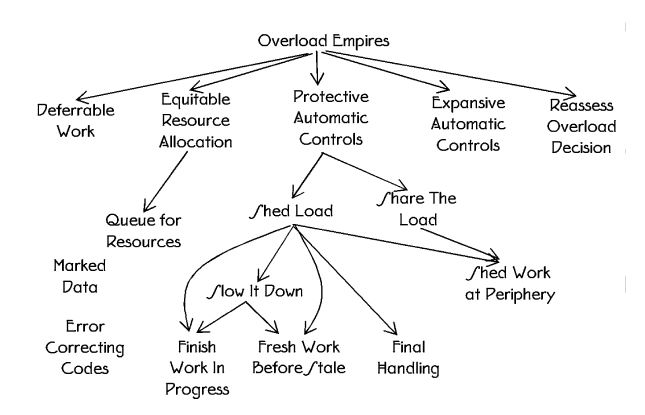
\includegraphics[width=\textwidth]{content/faulttolerance/images/MitigationPatterns_Dependecy.JPG}
	\caption{MitigationPatterns Dependecy}
\end{figure}


\begin{figure}[H]
	\centering
	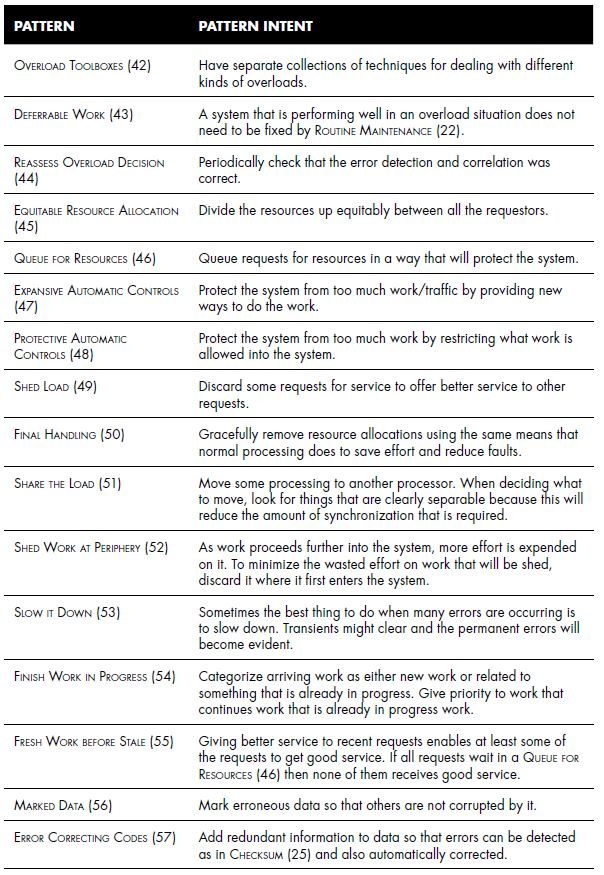
\includegraphics[width=\textwidth]{content/faulttolerance/images/MitigationPatterns.JPG}
	\caption{MitigationPatterns}
\end{figure}




\subsection{Overload Toolboxes}

\subsubsection*{Ausgangslage}

Das System stellt einen Fehler fest, erkennt aber, dass es sich nicht um einen Bug in der Hard- oder Software handelt sondern dieser ist entstanden durch zu viele Anfragen.

\subsubsection*{Lösungsansatz}

Zu viele Anfragen können ein System auf drei verschiedene Arten beeinträchtigen:
\begin{enumerate}
	\item \textbf{Memory:} Mehr Speicher wird benötigt um neue Anfragen zwischen zu speichern und abzuarbeiten. Dies kann dazu führen das aktuell abzuarbeitende Anfragen keinen Speicher mehr zur Verfügung haben.
	\item \textbf{Tangible (greifbar) Resources:} Anfragen können weitere, periphere Ressourcen anfordern, die aber noch durch eine frühere Anfrage blockiert sind. Dies kann zu Verzögerungen in der Verarbeitung und zu weiteren Fehler führen.
	\item \textbf{Processor CPU Time:} Anfragen abzuarbeiten kann mehr Zeit in Anspruch nehmen als dem System zu Verfügung stehen. Dies führt dazu, dass Anfragen nicht mehr (richtig) verarbeitet werden können.
\end{enumerate}

Falls diese Probleme in eine Knoten eines Netzes auftreten, kann auch eine Strategie entwickelt und umgesetzt werden, bei der, der entsprechende Knoten seine Nachbarn über die Überlastung informiert und diese ihm bei der Verarbeitung helfen können.

\subsubsection*{Schlussfolgerung}

Verwende mehrere Toolboxes um jedes Problem auf die bestmögliche Art abzuschwächen. Eine Toolbox soll sich um Buffer und Ports kümmern, die vom System verwaltet werden. Eine andere soll sich um den Speicher kümmern und eine weitere um die CPU. Vermeide Toolboxes, die mehrere Probleme versuchen zu lösen, da diese kaum eines richtig behandeln können.

\subsubsection*{Verwandte Patterns}

Anwendung bei zu wenig Ressourcen:
\begin{itemize}
	\item Queue for Resources (46)
	\item Equitable Resource Allocation (45)
	\item Finish Work in Progress (54)
\end{itemize}

\begin{itemize}
	\item Fresh Work before Stale (55)
	\item Share the Load (51)
	\item Shed Load (49)
	\item Finish Work in Progress (54)
\end{itemize}


\subsection{Deferrable Work}

\subsubsection*{Ausgangslage}

Ein System hat übermässig viele Anfragen. Um den korrekten Betrieb sicher zu stellen werden Routine Audits (24) und Routine Maintenance (22) angewandt. Durch die höhere Belastung des Systems treten aber keine Fehler auf, die behandelt werden müssen, lediglich die Ressourcen werden knapper.

\subsubsection*{Lösungsansatz}

Ist ein System stabil und steht es vor einer Überlastung, kann es Sinn machen, die Prüfungen, welche Fehler verhindern sollen, später als geplant durchzuführen. Denn diese Routine-Checks sind nicht wichtig für das Abarbeiten der Anfragen. Das System soll sich bei einer Überlastung auf seine primäre Funktionalität konzentrieren.

\subsubsection*{Schlussfolgerung}

Routinearbeit kann aufgeschoben (deferred) werden. Bei einem System, welches vor einer Überlastung steht, ist die Wahrscheinlichkeit gross, dass alle Komponenten richtig funktionieren. Die Routinearbeit soll dann wieder einsetzten, wenn die Ressourcen wieder vorhanden sind.

\begin{figure}[H]
	\centering
	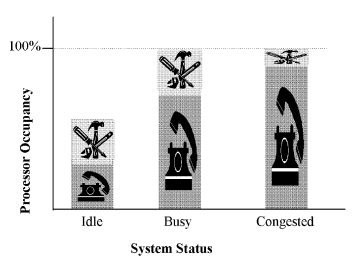
\includegraphics[width=\textwidth]{content/faulttolerance/images/DeferrableWork.JPG}
	\caption{DeferrableWork}
\end{figure}


\subsubsection*{Verwandte Patterns}

Falls ein Fehler Überlastung verursacht:
\begin{itemize}
	\item Reasses Overload Decision (44)
\end{itemize}




\subsection{Reassess Overload Decision}

\subsubsection*{Ausgangslage}

Ein System verwendet Fault Correlation (12), um eine Überlastung abzuwenden. Deshalb wird Deferrable Work (43), Finish Work in Prograss (54) und Shed Load (49) angewandt. Die Überlastung verringert sich aber nicht.

\subsubsection*{Lösungsansatz}

Falls erkannt wird, dass die Überlastung trotz der Versuche diese abzuwenden gleich bleibt oder gar zunimmt, kann es sein, dass die Überlastung nur eine Effekt eines Fehlers ist, der behandelt werden muss. Nimmt die Überlastung zu, muss dies im System festgestellt werden können um weitere respektive andere Massnahmen zu ergreifen.

\subsubsection*{Schlussfolgerung}

Es soll ein Feedback-Loop vorhanden sein, der es ermöglicht, die gefällten Entscheidungen zu korrigieren. Dies ermöglicht es dem System, eine andere Fehlerbehandlung durchzuführen, falls der gewünschte Effekt durch die gewählte Strategie nicht erreicht wird.

\begin{figure}[H]
	\centering
	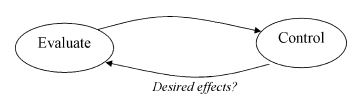
\includegraphics[width=\textwidth]{content/faulttolerance/images/ReassessOverloadDecision.JPG}
	\caption{ReassessOverloadDecision}
\end{figure}


\subsubsection*{Verwandte Patterns}

Anwendung von:
\begin{itemize}
	\item Escalation (9)
\end{itemize}

\begin{itemize}
	\item Someone in Charge (8)
\end{itemize}




\subsection{Equitable Resource Allocation}

\subsubsection*{Ausgangslage}

Verschiedene Typen von Anfragen werden von einem System behandelt. Hinzu kommt noch, dass diese unterschiedlich priorisiert sein können. Das System muss verhindern, dass es zusammenbricht, auch wenn nur ein Typ oder Priorität zur Überlastung neigt.

\subsubsection*{Lösungsansatz}

Als Beispiel nehmen wir Anfragen an eine Firmen-Webseite. Einige wollen nur Informationen abgreifen, andere Bestellungen platzieren. Zudem sollen Anfragen von Angestellten mit höherer Priorität behandelt werden als jene von Kunden.
Würde man nun strikt nach Fresh Work before Stale (55) vorgehen, würde dies bedeuten, dass immer die neuste Anfrage verarbeitet wird. Dies kann aber dazu führen, dass höher priorisierte Anfragen tiefer priorisierten weichen müssen. Das führt dann zu einer Priority-Inversion, falls tiefer priorisierte Anfragen Ressourcen blockieren, welche von höher priorisierten benötigt werden.
Eine andere Lösung wäre, basierend auf den eingehenden und bereits vorhandenen Anfragen die Ressourcen zu verteilen. So können so viele Anfragen wie möglich mit den vorhandenen Ressourcen verarbeitet werden und Überlastungen blockieren nicht alle Typen und Prioritäten von Anfragen.

\subsubsection*{Schlussfolgerung}

Bündle ähnliche Anfragen zusammen und stelle ihnen Ressourcen nach ihren Prioritäten bereit. Dies ermöglicht das Verarbeiten von allen Typen von Anfragen, auch wenn einige Gruppen zur Überlastung neigen.

\begin{figure}[H]
	\centering
	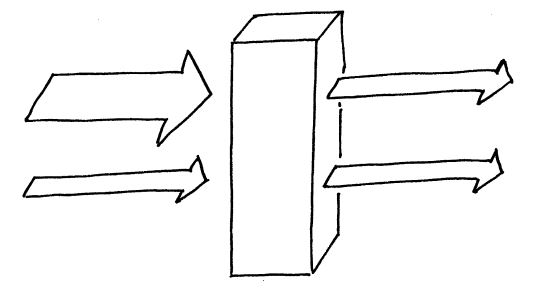
\includegraphics[width=\textwidth]{content/faulttolerance/images/EquitableResourceAllocation.JPG}
	\caption{EquitableResourceAllocation}
\end{figure}


\subsubsection*{Verwandte Patterns}

Anwendung:
\begin{itemize}
	\item Queue for Resources (46)
\end{itemize}


\subsection{Queue For Resources}

\subsubsection*{Ausgangslage}

Ein System versucht eine Überlastung zu verhindern. Es ist aber nicht mit einer Fehlerbehandlung beschäftigt sondern erhält einfach zu viele Anfragen.

\subsubsection*{Lösungsansatz}

Eine Möglichkeit wäre, nur die Anfragen zu behandeln, welche mit den freien Ressourcen behandelt werden können. Alle anderen werden verworfen. Shed Load (49) löst eine Überlastung so. Mit diesem Ansatz gibt es aber einige Probleme:
\begin{itemize}
	\item Eine Anfrage, welche sich aus mehreren kleineren Anfragen zusammensetzt, kann nicht abgeschlossen werden, weil eine Anfrage abgewiesen wurde.
	\item Wichtige Anfrage werden ohne Prüfung ignoriert (Siehe Maintenance Interface (7))
	\item Die Überlastung kann nur von kurzer Zeit sein und eine abgewiesen Anfrage könnte kurze Zeit später verarbeitet werden.
\end{itemize}

\begin{itemize}
	\item Die Queue wird zu lange, sodass sie nicht mehr verwaltet werden kann.
	\item Es stehen auch nach einer Weile nicht genügend Ressourcen für die vorderste Anfrage bereit und diese blockiert nun die Queue oder muss verworfen werden.
	\item Die Verwaltung der Queue benötigt zusätzliche Ressourcen und kann sehr ineffizient umgesetzt sein.
\end{itemize}

\subsubsection*{Schlussfolgerung}

Speichere Anfragen, die nicht direkt verarbeitet werden können, in einer Queue.

\begin{figure}[H]
	\centering
	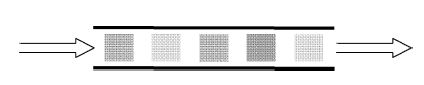
\includegraphics[width=\textwidth]{content/faulttolerance/images/QueueForResources.JPG}
	\caption{QueueForResources}
\end{figure}


\subsubsection*{Verwandte Patterns}

Queues:
\begin{itemize}
	\item FIFO (First In/First Out): Für Systemanfragen
	\item LIFO (Last In/First Out aka Stack): Für Anfragen von Benutzern. Derjenige, der als letztes die Anfrage abgesetzt hat, erhält am schnellsten Antwort. Derjenige, der als erstes eine Anfrage gestellt hat, hat wohl bereits aufgegeben.
\end{itemize}

\begin{itemize}
	\item Equitable Resource Allocation (45)
\end{itemize}



\subsection{Expansive Automatic Controls}

\subsubsection*{Ausgangslage}

Wie kann man es vermeiden Zeit unötig für nicht behandelbare Anfragen zu vergeuden und gleichzeitig andere Anfragen schnellst möglich abarbeiten?

\subsubsection*{Lösungsansatz}

Versuche das System so zu designen, dass bei Überlast alternative Wege genommen werden können. Dies könnte zu nicht Lastzeiten mit zusätzlichen Ressourcen erreicht werden, welche bei Last eingreifen können.

\subsubsection*{Schlussfolgerung}

Dieses Pattern versucht Zusatzwege in ein zu entwickelndes System einzubauen, welche eingeschlagen werden falls eine Grenze überschritten wird. Erst wenn die Überlast nicht trotz zusätzlicher Ressourcen nicht gelöst werden kann soll Shed Load (49) eingesetzt werden.

\subsubsection*{Verwandte Patterns}

Anwendung bei zu wenig Ressourcen:
\begin{itemize}
	\item Shed Load (49)
\end{itemize}


\subsection{Protective Automatic Controls}

\subsubsection*{Ausgangslage}

Wie soll das System mit dem Overhead von zu vielen Anfragen umgegangen werden die bearbeitet werden müssen?

\subsubsection*{Lösungsansatz}

Hierbei bestehen drei mögliche Ansätze:
\begin{enumerate}
	\item Versuche alles zu unternehmen um das System nicht zum Absturz zu bringen, dies könnte auch heissen keine Anfragen zu beantworten.
	\item Versuche so viele Anfragen wie möglich zu beantworten und lass dabei unnötige Vorberitungsarbeiten weg.
	\item Mache gar nichts, was jedoch meist in Instabilität endet.
\end{enumerate}

Ein gutes Beispiel für dieses Pattern ist, ein Lichtsignal an der Einfahrtsrampe einer Autobahn, welches in Aktion tritt sobald die Autobahn anfängt zu verstopfen. Diese Pattern wird verwendet, wenn die Ressourcen begrenzt sind.


\subsection{Marked Data}

\subsubsection*{Ausgangslage}

Ein Fehler wurde entdeckte, kann aber nicht korrigiert werden. Wie kann dieser verhindert werden, dass er sich im System weiterverbreitet?

\subsubsection*{Lösungsansatz}

Falls der Fehler bereits im Speicher vorhanden ist, können die Error Correcting Codes des Speichers verwendet werden, um den Fehler zu erkennen. Wurde der Fehler nicht erkannt können die Daten beim ersten Gebrauch geprüft werden und als fehlerhaft markiert werden. Oftmals hilft eine Markierung nicht aus, da danach jeweils geprüft werden muss ob diese Markierung vorhanden ist oder nicht. Deshalb könnten wie im Beispiel des IEEE Standards für NaN, ein neuer Wert eingeführt werden der im Fehlerfall zur weiteren Verarbeitung weitergegeben wird. Dabei ist das Verhalten bei der weiteren Verarbeitung definiert, also wie sich das System Verhalten soll falls der Wert für eine Berechnung verwendet wird.

\subsubsection*{Schlussfolgerung}

Markiere fehlerhafte Daten und definiere geeignete Regeln für die Verwendung dieser Daten.


\subsection{Error Correcting Codes}

\subsubsection*{Ausgangslage}

Wie können Daten möglichst Fehlerfrei gehalten werden bzw. wie können fehlerhafte Daten möglichst schnell korrigiert werden?

\subsubsection*{Lösungsansatz}

Mit dem Checksum Ansatz kann das System relativ schnell erkennen ob Daten korrekt sind, jedoch nicht welcher Teil ungültig ist. Deshalb müssen zusätzlich Korrekturbits eingeführt werden, womit das System erkennen kann welcher Teil zerstört bzw. ungültig ist.

\subsubsection*{Schlussfolgerung}

Speichere mit jeder Checksum möglichst viele Informationen, damit fehlerhafte Daten möglichst korrigiert werden können.


\subsection{Shed Load}

\subsubsection*{Ausgangslage}

Wie können zu viele Anfragen an ein System bestmöglichst behandelt werden, ohne es in die Knie zu zwingen?

\subsubsection*{Lösungsansatz}

Es sollen frühstmöglich begonnen werden Anfragen abzuweisen, falls die Gefahr besteht das ein System anfängt zu überlasten. Dabei ist es wichtig sich zu vergewissern, dass das System dies gegen aussen richtig kommuniziert.

\subsubsection*{Schlussfolgerung}

Lehne gewisse Anfragen ab, um das System am laufen zu halten.


\subsection{Final Handling}

\subsubsection*{Ausgangslage}

Braucht es einen eigen Mechanismus um besetzte Ressourcen frei zu gegeben, welche von irregulär beendeten Prozessen besetzt sind?

\subsubsection*{Lösungsansatz}

Die einfachste Lösung wäre sich nicht um die Ressourcenfreigabe zu kümmern und falls vorhanden den Garbage Collector seine Arbeit machen lassen. Der bessere Ansatz ist jedoch zur Programmierzeit bereits einen Ressourcenfreigabemechanismus einzubauen, welcher bei normaler und irregulärer Beendigung von Prozessen zum Zuge kommt. Dies vereinfacht die Programmierung und stellt sicher das Ressourcen freigegeben wurden.

\subsubsection*{Schlussfolgerung}

Integriere das freigeben von Ressourcen in den normalen Programmfluss, so dass auch nach einem Fehler und dessen Behandlung genügend Ressourcen zur Verfügung stehen.


\subsection{Share the load}

\subsubsection*{Ausgangslage}


Das System soll grossen Workload bearbeiten können. Es besteht evtl. aus mehreren parallelen Elementen, z.B. in einem Cluster oder mit Multicore.

\subsubsection*{Frage}


Wie kann die verfügbare 'processing power' vergrössert werden?
Einfach Prozessoren hinzuzufügen erhöht die Komplexität. Auch muss man aufpassen, was mit Funktionalitäten in Mehrkernsystemen passiert. Wird dabei viel herum geschoben, so ergibt sich erheblichen Overload (Synchronisation etc.).

\subsubsection*{Lösungsansatz}


Lasse gewisse Arbeit von anderen Prozessoren erledigen. Wähle Arbeiten aus, welche nur geringen Synchronisationsaufwand benötigen.

\subsection{Slow it down}

\subsubsection*{Ausgangslage}


Gibt es keine gesetzten Limiten für Systemrequests, so kann das System im schlimmsten Fall mit Arbeit überladen werden, bis gar nichts mehr geht.

Das System kann im Grenzfall auch nicht auf menschliche Hilfe warten (s. Minimize Human Intervention)

\subsubsection*{Frage}


Was soll das System tun, wenn die Anzahl Requests die Effizienz zu beeinträchtigen drohen?
Ein Shutdown bringt nicht den gewünschten Erfolg, da das System ja nützliche Arbeit erledigen sollte.

\subsubsection*{Lösungsansatz}


Es gibt verschiedene Mechanismen um das System vom Overload zu befreien. Einige sind restriktiver als andere. Nutze daher eine Art von Escalation, um immer stärker auf die Bremse treten zu können, falls ein Mechanismus noch nicht den gewünschten Effekt bringt.

\subsection{Shed work at periphery}

\subsubsection*{Frage}


Wie kann man dem System, das mit Shed Load arbeitet, möglichst viel Arbeit abnehmen? Das belastete System sollte ja nicht noch mit zusätzlichem Arbeitsaufwand belastet werden.

\subsubsection*{Lösungsansatz}


Versuche zu verwerfende Requests so nahe der Systemgrenze wie möglich zu erkennen. Dies hilft dem Systemkern, sich auf die wirklich wichtigen Aufgaben konzentrieren zu können.

\subsection{Finish work in progress}

\subsubsection*{Ausgangslage}


Requests können in verschiedener Art und Weise miteinander in Beziehung stehen. Z.B. kann es sein, dass Requests auf früheren aufbauen.

Ansätze wie Slow it down und Shed load sind zwar im System eingebaut, scheinen aber nicht viel zu nützen.

\subsubsection*{Frage}


Welche Requests soll das System akzeptieren und welche verwerfen?
Besteht ein solcher z.B. aus mehreren Sub-Requests, so will man sicher nicht den letzten davon verwerfen, da sonst das System schon bald wieder mit dem ganzen Requestsatz bombardiert wird

\subsubsection*{Lösungsansatz}


Verarbeite zusammenhängende Requests (von denen der Super-Request schon verarbeitet wurde) und verwerfe solche, die neu ankommen.

\subsection{Fresh work before stale}

\subsubsection*{Ausgangslage}


Es kommen mehr Requests ins System rein, als es bearbeiten kann. Man möchte QoS jedoch so hoch wie möglich halten.
Der Benutzer ist in der Lage, Requests abzubrechen und neue zu starten (Beispiel: Webseiten-Requests).
Das System hat die Fähigkeit, eingehende Requests in unterschiedliche Kategorien zu sortieren. Dies ermöglicht dem System, FINISH WORK IN PROGRESS (54) sowie SHED LOAD (49) anzuwenden.

\subsubsection*{Frage}


Wie kann man sicherstellen, dass so viele Requests als möglich den bestmöglichen Service erhalten?

\subsubsection*{Lösungsansatz}


Wenn Requests sehr lange dauern, gibt der Nutzer meist auf und bricht ihn ab. Dies kann dazu führen, dass das System noch mehr zu tun hat, wenn es beispielsweise den Request startet und erst dann merkt, dass dieser bereits von der Userseite her abgebrochen wurde.
Wenn das System so viele Requests behandelt wie es nur kann, ist es dazu gezwungen, die Requests in einer Queue zu halten. Der einfachste Weg für eine Queue ist ein Buffer, welcher wie eine FiFo Queue funktioniert. Das Problem bei diesem Buffer ist jedoch, dass abgebrochene Requests erst dann entdeckt werden, wenn sie behandelt werden.

Requests können schnell behandelt werden, wenn ein Stack eingesetzt wird (LiFo-Queue). Dies ermöglich dem System, mit dem aktuellsten Requests zu arbeiten. Dies impliziert, dass es wahrscheinlicher ist, dass die Requests noch nicht abgebrochen wurden.

Wenn das System weiss, wie lange Requests warten bis sie abgebrochen werden, kann es besser entscheiden, welche Requests bearbeitet werden müssen. Es ist jedoch schwierig die Übersicht zu behalten, welche Requests bereits wie lange warten. Dies führt darüber hinaus auch zu mehr Overhead.


\section{Fault Treatment Patterns}


\begin{itemize}
	\item Wird ein Error mithilfe von \textbf{Detection Patterns} gefunden, wird das System entweder durch
	\begin{itemize}
		\item \textbf{Recovery Patterns} zurück in einen fehlerfreien Zustand überführt, oder der Error wird durch
		\item \textbf{Mitigation Patterns} maskiert, sodass die Auswirkungen so klein wie möglich gehalten werden
	\end{itemize}
	\item Nun kommen die \textbf{Fault Treatment Patterns} zum Einsatz; Es wird versucht, den Fault welcher den Error verursacht zu finden und zu korrigieren.
\end{itemize}



\begin{figure}[H]
	\centering
	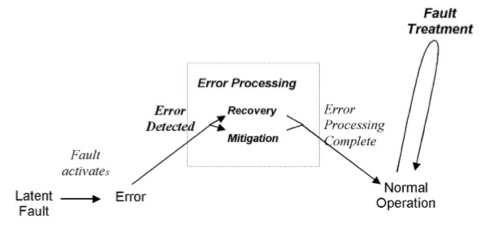
\includegraphics[width=\textwidth]{content/faulttolerance/images/fault_treatment.png}
	\caption{fault treatment}
\end{figure}




Um einen Fault mithilfe der \textbf{Fault Treatment Patterns} zu eliminieren, werden folgende Schritte durchloffen:
\begin{itemize}
	\item \textbf{Verification}
	\begin{itemize}
		\item Es wird geprüft, ob sich das System gemäss seiner Spezifikation verhält. Dies wird gemacht um zu prüfen, ob sich der Fault (immer noch) im System befindet.
	\end{itemize}
	\item \textbf{Diagnosis}
	\begin{itemize}
		\item Die Ursache des Fehlers wird untersucht. Es gilt, den Fault welcher zum Error führt, aufzuspüren und die genaue Erscheinungsform des Errors zu erforschen.
	\end{itemize}
	\item \textbf{Correction}
	\begin{itemize}
		\item Der Fehler wird aus dem System entfernt. (Sourcecode, System-Konfiguration etc.)
	\end{itemize}
	\item \textbf{Verification} \#2
\end{itemize}

\subsection*{Prüfungsfragen}

\begin{itemize}
	\item Was ist das Ziel von Fault Treatment Patterns?
	\item Welche Schritte werden beim Einsatz von Fault Treatment Patterns durchloffen?
\end{itemize}


\subsection{Let Sleeping Dogs Lie}


\subsubsection*{Problem}


Das System hat einen Error detektiert und ihn anschliessend korrigiert (Error Processing Patterns: Recovery oder Mitigation). Nun geht es darum, den Fault, welcher den Error aktiviert hat, zu korrigieren.

\subsubsection*{Lösung}


\begin{itemize}
	\item \textbf{Sollen alle Faults, welche vom System oder von einem Entwickler gefunden wird, behoben werden?}
\end{itemize}

Diese Frage lässt sich nicht generell beantworten! Einen Fehler in einem Software-System zu beheben verhält sich ähnlich wie ein medizinischer Eingriff. Der Eingriff an einem Patienten (die Software), birgt immer ein gewisses Risiko für Komplikationen. Deshalb muss vor einem solchen Eingriff geprüft werden, ob sich dieser überhaupt sinnvoll ist.

Dabei werden die Vorteile/Belohnung des Bugfixing den Kosten/Risiken gegenübergestellt. Folgende Fragen helfen bei der Entscheidung, ob ein bekannter Fault korrigiert werden sollte oder nicht:

\begin{itemize}
	\item Welchen Risiken setzen wir das System aus, wenn der Fault nicht korrigiert wird?
	\item Wie stark wird das System durch die Fehlerbehebung verkompliziert?
	\item Wie gross ist die Wahrscheinlichkeit dass der Fehler korrigiert wird, ohne neue Fehler zu verursachen?
	\item Wie gross ist die Wahrscheinlichkeit, dass die Software neu installiert wird, ohne neue Fehler zu verursachen?
	\item Was kostest es uns neue Tests zu schreiben?
	\item Was kostet es uns den Fehler zu beheben und anschliessend erneut zu testen?
	\item Was kostet es uns eine verbesserte Software zu erstellen und anschliessend zu deployen?
	\item Wie teuer ist die Downtime des Systems, während gepatched wird?
\end{itemize}

Je nach dem entscheiden Sie sich den Fault zu suchen und zu beheben, oder Sie entscheiden sich den schlafenden Hund liegen zu lassen ;-)

\subsubsection*{Prüfungsfragen}

\begin{itemize}
	\item Welche Faktoren stellen Sie einander gegenüber, wenn Sie entscheiden müssen ob ein neu entdeckter Fault korrigiert werden soll?
	\item Was ist mit \textbf{Let Sleeping Dogs Lie} gemeint? Erläutern Sie.
\end{itemize}


\subsection{Reproducible Error}


\subsubsection*{Problem}


Es ist ein Fehler aufgetreten. Durch Error-Mitigation konnte das System weiterlaufen. Nun geht es darum, den Fehler zu korrigieren. Zum Glück müssen wir nicht bei Null beginnen, sondern haben Informationen über den Fehler, welche vom System geloggt wurden.

Es ist wichtig, den eigentlichen Fehler zu behandeln und sich nicht mit einem eingebildeten Fehler zu versäumen. Das System ist nicht in einem statischen Zustand; seit dem Auftreten des Fehlers kann sich das System verändert haben. Vielleicht gab es unterdessen ein Software Update durch welches als Seiteneffekt der Fehler bereits behoben wurde.
Ausserdem muss sichergestellt werden, dass derjenige Fault behandelt wird, der den konkreten Error oder Failure auch wirklich ausgelöst hat.

\subsubsection*{Lösung}


Löse auf kontrollierte Art und Weise den Fehler aus, um sicherzustellen, dass auch wirklich ein Fehler existiert. Dabei sollte das so beobachtete Verhalten mit der Systemspezifikation verglichen werden. Ein Fault wurde erst identifiziert wenn dieser mit bekannten Stimuli immer wieder reproduziert werden kann!

\subsubsection*{Trade-off}


Die Fehlersuche kann sehr zeitintensiv sein! Faults sind nicht nur im Quellcode zu suchen; Die Kombination aus Hardware, Software und Konfiguration muss untersucht werden.


\subsection{Small Patches}


\subsubsection*{Problem}


Es gibt einen bekannten Fehler der zu beheben ist. Die Option LETTING SLEEPING DOGS LIE wurde ausgeschlossen. Es ist bekannt, wie der Fehler korrigiert werden kann.

Es geht nun darum, die Ausfallzeit des Systems und das Risiko für neu eingeführte Fehler zu minimieren. Je grösser das Update ist, je grösser der Codeumfang des Updates ist, um so grösser ist die Komplexität und umso mehr Möglichkeiten gibt es, einen neuen Fehler einzubauen. Ausserdem steigt der Aufwand für die Entwicklung und das Testen.

\subsubsection*{Lösung}


Mache Updates so klein wie möglich. Dies hängt von den Tools und dem zu patchenden Bug ab.

\subsubsection*{Trade-off}


Es ist nicht immer möglich, ein Patch in ein laufendes System einzuspielen. Sind keine ``Hot Deployment''-Mechanismen vorhanden, muss das System neu gestartet werden.

Bei einem System ohne physischen Zugriff besteht die Gefahr, dass nach einem fehlerhaften Path nicht mehr darauf zugegriffen werden kann!

\subsection{Root Cause Analysis}


\subsubsection*{Problem}


Der Fehler (fault) A wird zum Error (error) A und führt zum System Fehler (failure) A. Dieser führt zu Fehler B. Fehler B wird zum Error und führt zum System Fehler B. Dies kann unter Umständen immer so weiter gehen, dabei werden die einzelnen Fehler vom System geloggt. Das System hat inzwischen den Fehler behoben und arbeitet normal weiter. Jetzt ist es an der Zeit den Fehler zu analysieren und zu beheben, welcher den Error verursacht hat.

\begin{figure}[H]
	\centering
	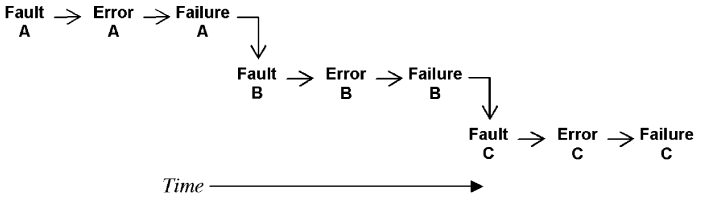
\includegraphics[width=\textwidth]{content/faulttolerance/images/failureSequence.PNG}
	\caption{failureSequence}
\end{figure}


Wie bereits angedeutet, kann der erkannte Error die Ursache für weitere Failure sein. Und umgekehrt, kann ein Error auch mehrere Faults als Vorgänger haben.

\subsubsection*{Lösung}


\begin{figure}[H]
	\centering
	
\includegraphics[width=\textwidth]{content/faulttolerance/images/why.png}
	\caption{why}
\end{figure}


Um einen Error zu beheben muss das Problem bei der Wurzel gelöst werden, also beim ursprünglichen Verursacher des Errors, auch root cause genannt. Dieser Fault muss als erstes korrigiert werden. Danach werden alle weiteren Faults nach und nach bis zum verursachenden Fault korrigiert. Um den sogenannten root cause zu finden, kann die 5 Warum-Fragetechnik verwendet werden.

\begin{itemize}
	\item Why was the data record lost?
	\begin{itemize}
		\item Because the transaction failed in the middle.
	\end{itemize}
	\item Why did the transaction fail in the middle?
	\begin{itemize}
		\item Because it ran out of memory.
	\end{itemize}
	\item Why did it run out of memory?
	\begin{itemize}
		\item Because there was no more memory available for allocation.
	\end{itemize}
	\item Why was there no more memory available for allocation?
	\begin{itemize}
		\item Because the memory was inaccessible.
	\end{itemize}
	\item Why was the memory inaccessible?
	\begin{itemize}
		\item Because its owning task had terminated without releasing it.
	\end{itemize}
\end{itemize}

Am Ende dieser Kette haben wir den ursprünglichen Auslöser gefunden. Es kann auch sein das es mehrere dieser Auslöser gibt.

\subsection{Revise Procedure}


\subsubsection*{Problem}


Nach einem Failure wurden die Faults mit Root Cause Analysis gefunden und mit einem Update gelöst. Die Root Cause Analysis hat jedoch herausgefunden, dass die Failures durch menschliche Fehleinschätzungen bei der Programmierung oder der Wartung entstanden. Daher sollten Produktionsabläufe konzipiert werden, welche den Operators diese Fehler nicht ermöglichen.

\subsubsection*{Lösung}


Experten wissen was sie eingeben müssen, weil diese das System sehr gut kennen (Entwickler). Jedoch ist nicht jeder Operator solch ein Experte:
\begin{itemize}
	\item Falls ein „nichtexperte“ Fehlermeldungen falsch interpretiert, so kann dieser mit seinem Fix ein anderes Problem hervorrufen.
	\item Schlechte Instruktionsanweisungen führen zu willkürlichem Trial and Error und den daraus folgenden Miskonfigurationen.
\end{itemize}

Testen der Manuals, sowie verbessern der Manuals führt zu weniger menschlichen Fehlern.


\subsubsection*{Beispiel}

\begin{itemize}
	\item Checklisten im Flugverkehr
\end{itemize}


